\documentclass[handout]{beamer}
\setbeamertemplate{section in toc}[sections numbered]
\setbeamertemplate{subsection in toc}[subsections numbered]
\usetheme[titlepagelogo=logo_ucla_seal, secondlogo=logo_ucla_cw, language=english]{TorinoTh}
\usepackage{hyperref}% http://ctan.org/pkg/hyperref
\hypersetup{%
  colorlinks = true,
  linkcolor  = black
}                                        
\usepackage[beamer,customcolors]{hf-tikz}
\usepackage{amsmath}
\usepackage{amssymb}
\usepackage{mathtools}
\usepackage{array}
%\usepackage[natbib=true]{biblatex}

\usepackage{amsthm}
\usepackage{amsmath}
\usepackage{amssymb}
\usepackage{bbm}
\usepackage{mathtools}
\usepackage{subfigure}
\usepackage{placeins}
\usepackage{import}
\usepackage{graphics}
\usepackage{graphicx}
\usepackage{tabularx}
\usepackage{bm}
\usepackage{booktabs}
\usepackage{todonotes}
\usepackage{color}
\usepackage{array}
\usepackage{natbib}
\usepackage[toc,page]{appendix}
\usepackage{floatrow}
\usepackage{color, colortbl}
\usepackage{placeins} % for FloatBarrier
\usepackage{algorithm}
\usepackage{algorithmic}
\usepackage{chapterbib}
\definecolor{Gray}{gray}{0.9}
\DeclareMathAlphabet{\mbf}{OT1}{ptm}{b}{n}

\theoremstyle{definition}
\newtheorem{conj}{Conjecture}[section]
\newtheorem{prop}{Proposition}[section]
\newtheorem{notation}{Notation}
\def\newblock{\hskip .11em plus .33em minus .07em}

\graphicspath{{}}
\makeatletter
\newcommand\appendtographicspath[1]{%
  \g@addto@macro\Ginput@path{#1}%
}
\makeatother

\def\p{\ensuremath{\mathbf{p}}}
\def\v{\ensuremath{\mathbf{v}}}
\def\x{\ensuremath{\mathbf{x}}}
\def\one{\mathbbm{1}}
\def\eps{\varepsilon}

\def\RR{\mathbb{R}}
\def\HH{\mathbb{H}}
\def\PP{\mathbb{P}}
\def\NN{\mathbb{N}}
\def\EE{\mathbb{E}}
\def\II{\mathbb{I}}

\def\A{\mathcal{A}}
\def\Y{\mathcal{Y}}
\def\O{\mathcal{O}}
\def\U{\mathcal{U}}
\def\P{\mathcal{P}}
\def\I{\mathcal{I}}
\def\L{\mathcal{L}}
\def\D{\mathcal{D}}
\def\V{\mathcal{V}}
\def\C{\mathcal{C}}
\def\R{\mathcal{R}}
\def\S{\mathcal{S}}
\def\T{\mathcal{T}}

\def\del{\partial}
\def\1{^{\prime}}
\def\neg{\mathord{\sim}}
\def\qtx#1{\quad\text{#1}\quad}
\def\subs{\subseteq}
\def\andn{\smallsetminus}

\def\IPV{\I_{\operatorname{Poisson}}}


%opening
\def\sscale{0.7}
%\def\tT{\widetilde\T}
\def\tT{\T\1}

\def\nop{\text{nop}}
\def\ang#1{\left\langle#1\right\rangle}
\def\inv{^{-1}}

\def\seq{\operatorname{Sequences}}
\def\Rep{\operatorname{Rep}}
\def\Comp{\operatorname{Comp}}
\def\Adj{\operatorname{Adj}}

\renewcommand{\algorithmicrequire}{\textbf{Input:}}
\renewcommand{\algorithmicensure}{\textbf{Output:}}
\hfsetfillcolor{alerted text.fg!10}
\hfsetbordercolor{alerted text.fg}

\author{Josh Hernandez}
\rel{Stefano Soatto}
\title{Models and Methods for Sensor-Based
Environment Exploration}
\ateneo{University of California, Los Angeles}
\date{\today}

\AtBeginSection[]
{
  \begin{frame}<beamer>
    \frametitle{Outline for section \thesection}
    \tableofcontents[currentsection]
  \end{frame}
}

\begin{document}
\titlepageframe

\begin{tframe}{Overview}
How to endow a robot with a ``sense'' of the surrounding environment?
\begin{description}
 \item<2->[Localization] To interact with the environment, I need to know where I am, relative to where I have been and what I have seen.
 \item<3->[Mapping] Once I we know where I am, I need to know the affordances of the things around me.
 \item<4->[Exploration] Once I know the objects around me, I can expand my region of understanding.
 \item<5->[Representation] As that region grows, I must compress my understanding to fit my mind.
\end{description}
\end{tframe}
\begin{tframe}{Outline of the Talk}
\tableofcontents
\end{tframe}
\section{Overview}
\subsection{Observability of Visual-Inertial Navigation}
\newcommand{\be}{\begin{equation}}
\newcommand{\ee}{\end{equation}}
\newcommand{\ba}{\left[ \begin{array}}
\newcommand{\ea}{\end{array} \right]}
\newcommand{\bea}{\begin{eqnarray}}
\newcommand{\eea}{\end{eqnarray}}
\newcommand{\bc}{\begin{cases}}
\newcommand{\ec}{\end{cases}}
\newcommand{\psfigure}[3]
        {
        \begin{tabular}{c}
        { \psfig{figure=#1,height=#2in,width=#3in}}
        \end{tabular}   }

\def\real{\mathbb{R}}
\def\X{{\mathbf{X}}}
\def\x{{\mathbf{x}}}
\def\w{\omega}
\def\hw{{\widehat\w}}
\def\ww{\tilde\w}
\def\hww{\widehat\ww}

\newtheorem{defn}{Definition}
\newtheorem{rem}{Remark}
\newtheorem{claim}{Claim}

\def\gw{\tilde{g}}
\def\Xw{\tilde{X}}
\def\Rw{\tilde{R}}
\def\Tw{\tilde{T}}
\def\1{^{\prime}}

\def\g{g}
\def\inv{^{-1}}
\def\RR{\mathbb{R}}
\def\s{\sigma}
\def\sit{\s_{i}}
%\def\dot#1{\tfrac{d#1}{dt}}
\def\dX{\delta X}
\def\subs{\subset}
\def\andn{\smallsetminus}
\def\Mm{\mathcal{M}}
\def\SO{\operatorname{SO}}
\def\SE{\operatorname{SE}}
\def\so{\mathfrak{so}}
\def\se{\mathfrak{se}}
\def\Aa{\mathcal{A}}
\def\ignore#1{}
\def\imu{_\mathrm{imu}}
\def\m{{m}}
\def\M{{M}}
\def\I{\mathcal{I}}

%\def\cut#1{{ #1}}
\def\cut#1{{}}

%\begin{abstract}
%\end{abstract}

\begin{tframe}{IMU Dynamics - stationary}
\begin{equation}
\begin{cases}
\begin{tabular}{>{$}r<{$} >{$\!\!\!\!\!}l<{$} >{$}r<{$} >{$\!\!\!\!\!}l<{$}}
\dot T &= V & T(0) &= 0 \\
\dot R &= R \widehat \w & R(0) &= R_0\\
\dot V &= \alpha \\ %~~~~~~ V(0) = V_0 \\
\dot \w &= w\\ % ~~~~~~~ \w(0) = \w_0 \\
\dot \alpha &= \xi \\% ~~~~~~ \alpha(0) = \alpha_0 \\
\dot \w_b &= n_{\w_b}  \\
\dot \alpha_b &= n_{\alpha_b}  \\ 
\dot \gamma &= 0 \\
\end{tabular}\\
\begin{tabular}{>{$}r<{$} >{$\!\!\!\!\!}l<{$}}
\w\imu (t) &= \w(t) + \alert<2>{\w_b(t)} + n_{\w}(t) \\ 
\alpha\imu (t) &= R^T(t) (\alpha(t)- \gamma) + \alert<2>{\alpha_b(t)} + n_{\alpha}(t) 
\end{tabular}
\end{cases}
\end{equation}
\end{tframe}
 
\begin{tframe}{Bounds on Indistinguishable Set}
\begin{claim}[Indistinguishable Trajectories from IMU Data]\label{claim-five}
Let $g(t)= (R(t), T(t)) \in \SE(3)$ be such that
\begin{equation}
\begin{cases}
\begin{tabular}{>{$}r<{$} >{$\!\!\!\!\!}l<{$}}
\dot R &= R(\hw\imu  - \hw_b) \\
\dot T &= V \\
\dot V &= R(\alpha\imu  - \alpha_b) + \gamma
\end{tabular}
\end{cases}
\label{eq-model-dyn}
\end{equation}
for some known constant $\gamma$ and functions $\alpha\imu (t)$, $\w\imu (t)$ and for some unknown functions $\alpha_b(t), \w_b(t)$ that are constrained to have $\| \dot \alpha_b(t) \| \le \epsilon$, $\| \dot \w_b(t) \| \le \epsilon$, and $\|\ddot\w_b(t)\|\le\epsilon$ at all $t$,
for some $\epsilon<1$.
\end{claim}
\end{tframe}

\begin{tframe}{Bounds on Indistinguishable Set}
\begin{claim}[continued]
Suppose $\gw(t) \doteq \sigma(g_B g(t) g_A)$ for some  constant $g_{A,B} = (R_{A,B}, T_{A,B})$, $\sigma > 0$,
$\|T_A\|\leq M_A$ and $|\sigma|\leq M_\sigma$.
Then, with sufficient excitation,
\begin{gather*}
\| I - R_A \|  \leq  \frac{2{\epsilon}}{\alert<2>{\m(\dot{\w}\imu\!:\!{\RR^+})}}  \label{constraint1}\\
|\sigma - 1|  \le \frac{k_{c_1}\epsilon + M_\sigma\|I-R_A\|}{\alert<3>{\M(\dot\alpha\imu\!:\!{\I_{c_1}})}} \label{constraint2}\\
\|T_A\|\leq \frac{\epsilon(k_{c_2}+(2M_\sigma+1)M_A)}{(1-|\sigma-1|)\,\alert<2>{\m(\ddot\w\imu\!:\!{\I_{c_2}})}}\label{constraint3} \\
\|(1-R_B^T)\gamma\|\leq\frac{\epsilon(k_{c_3} + M_\sigma M_A) + (|\sigma-1|+\epsilon)\alert<3>{\M(\w\imu-\w_b\!:\!\I_{c_3})}\|\gamma\|}
{\alert<2>{\m(\w\imu-\w_b\!:\!\I_{c_3})}\,(1-|\sigma-1|)}\label{constraint4}
\end{gather*}
\end{claim}
\end{tframe}



\subsection{Scene Segmentation by Aggregation of Global Ordering Constraints}
\begin{tframe}{Pipeline}

\bigskip
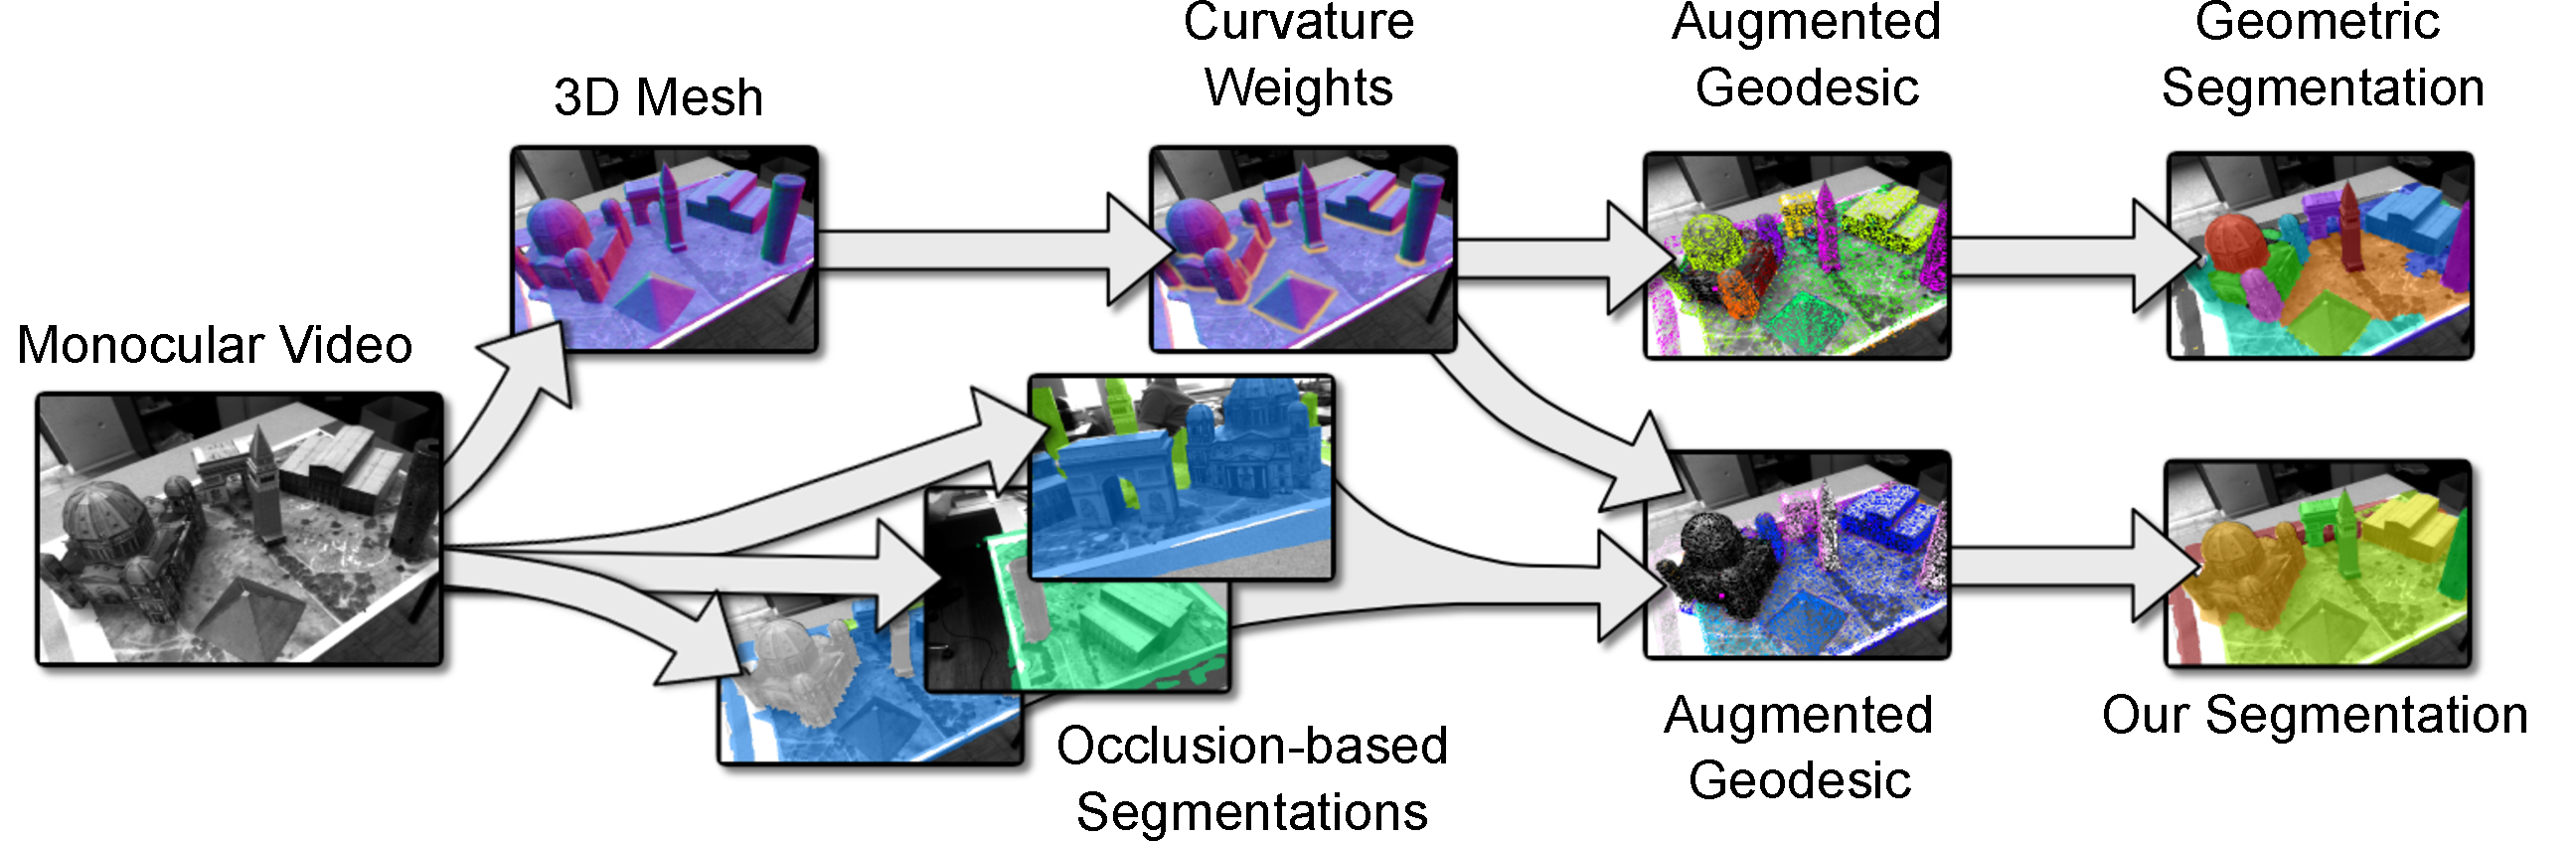
\includegraphics[width=4in]{media_solobj/pipeline}
\end{tframe}

\begin{tframe}{VIDEO}
\end{tframe}

\begin{tframe}{Comparisons}
\resizebox{.9\textwidth}{!}{
\begin{tabularx}{8in}{r *{4}{cc}}
\toprule
& \multicolumn{2}{c}{\emph{City of Sights}}
& \multicolumn{2}{c}{\emph{Pipes1}}
& \multicolumn{2}{c}{\emph{Pipes2}}
& \multicolumn{2}{c}{\emph{Tree}}\\
& Frame & Scene & Frame & Scene & Frame & Scene & Frame & Scene\\
\cmidrule(lr){2-3} \cmidrule(lr){4-5} \cmidrule(lr){6-7} \cmidrule(lr){8-9}
CGAL
\footnote{ L. Shapira, A. Shamir, and D. Cohen-Or. Consistent mesh
partitioning and skeletonisation using the shape diameter
function. \emph{Vis. Comput.}, 24(4):249–259, Mar. 2008} 
\begin{tabular}{r} F-Score \\ Precision \\ Recall \end{tabular} & 
\begin{tabular}{c} $.803\pm.041$ \\ $.822\pm.043$ \\ $.785\pm.041$ \end{tabular} & 
\begin{tabular}{c} .787 \\ .798 \\ .776 \end{tabular} &

\multicolumn{2}{c}{Fails} &

\begin{tabular}{c} ${\bm{.915\pm.032}}$ \\ $.959\pm.036$ \\ $.875\pm.041$ \end{tabular} &
\begin{tabular}{c} ${\bm{.869}}$ \\ .903 \\ .838 \end{tabular} &

\begin{tabular}{c} $.643\pm.049$ \\ $.633\pm.058$ \\ $.657\pm.053$ \end{tabular} &
\begin{tabular}{c} .604 \\ .608 \\ .599 \end{tabular}\\
\midrule

WCSeg
\footnote{O. van Kaick, N. Fish, Y. Kleiman, S. Asafi.
Shape segmentation by approximate convexity analysis.
\emph{ACM Trans. on Graphics, 2014}.}
\begin{tabular}{r} F \\ P \\ R \end{tabular} & 
\begin{tabular}{c} $.775\pm.028$ \\ $.938\pm.033$ \\ $.661\pm.033$ \end{tabular} & 
\begin{tabular}{c} .732 \\ .912 \\ .612 \end{tabular} &

\begin{tabular}{c} ${\bm{.730\pm.030}}$ \\ $.843\pm.040$ \\ $.645\pm.036$ \end{tabular} & 
\begin{tabular}{c} ${\bm{.725}}$ \\ .841 \\ .637 \end{tabular} &

\begin{tabular}{c} $.738\pm.045$ \\ $.820\pm.050$ \\ $.676\pm.068$ \end{tabular} &
\begin{tabular}{c} .730 \\ .904 \\ .612 \end{tabular} &

\begin{tabular}{c} $.806\pm.027$ \\ $.885\pm.031$ \\ $.742\pm.038$ \end{tabular} &
\begin{tabular}{c} .747 \\ .889 \\ .644 \end{tabular}\\
\midrule

\begin{tabular}{c} Ours \\ (Geom. only) \end{tabular} \begin{tabular}{r} F \\ P \\ R \end{tabular} & 
\begin{tabular}{c} ${\bm{.923\pm.018}}$ \\ $.986\pm.018$ \\ $.867\pm.020$ \end{tabular} & 
\begin{tabular}{c} ${\bm{.788}}$ \\ .866 \\ .722 \end{tabular} &

\begin{tabular}{c} $.705\pm.036$ \\ $.761\pm.043$ \\ $.658\pm.040$ \end{tabular} & 
\begin{tabular}{c} .648 \\ .690 \\ .612 \end{tabular} &

\begin{tabular}{c} $.818\pm.045$ \\ $.820\pm.056$ \\ $.818\pm.047$ \end{tabular} &
\begin{tabular}{c} .701 \\ .751 \\ .657 \end{tabular} &

\begin{tabular}{c} $.720\pm.036$ \\ $.763\pm.036$ \\ $.683\pm.041$ \end{tabular} &
\begin{tabular}{c} .729 \\ .783 \\ .681 \end{tabular}\\
\midrule

\begin{tabular}{c} Ours \\ (Geom. + Vis.) \end{tabular} \begin{tabular}{r} F \\ P \\ R \end{tabular} & 
\begin{tabular}{c} $.870\pm.043$ \\ $.853\pm.028$ \\ $.888\pm.062$ \end{tabular} & 
\begin{tabular}{c} .767 \\ .763 \\ .770 \end{tabular} &

\begin{tabular}{c} $.662\pm.027$ \\ $.689\pm.040$ \\ $.637\pm.030$ \end{tabular} & 
\begin{tabular}{c} .605 \\ .611 \\ .599 \end{tabular} &

\begin{tabular}{c} $.804\pm.063$ \\ $.810\pm.064$ \\ $.800\pm.072$ \end{tabular} &
\begin{tabular}{c} .648 \\ .679 \\ .620 \end{tabular} &

\begin{tabular}{c} ${\bm{.828\pm.034}}$ \\ $.803\pm.028$ \\ $.856\pm.032$ \end{tabular} &
\begin{tabular}{c} ${\bm{.836}}$ \\ .790 \\ .888 \end{tabular}\\
\midrule

\end{tabularx}}
\end{tframe}


\begin{tframe}{Contribution}
\begin{itemize}
 \item First bounds on indistinguishable set with IMU bias drift.
 \item Developed system for video segmentation leveraging image-plane segmentations.
\end{itemize}
\end{tframe}
\subsection{Desiging Agents with Task-Specific Minimal Representation}
\begin{tframe}{VIDEO}
\end{tframe}

\section{Featured Chapter: Information-Driven Autonomous Exploration}
\begin{tframe}{Autonomous Exploration}

\bigskip
\begin{tabular}{cl}
\begin{tabular}{c}
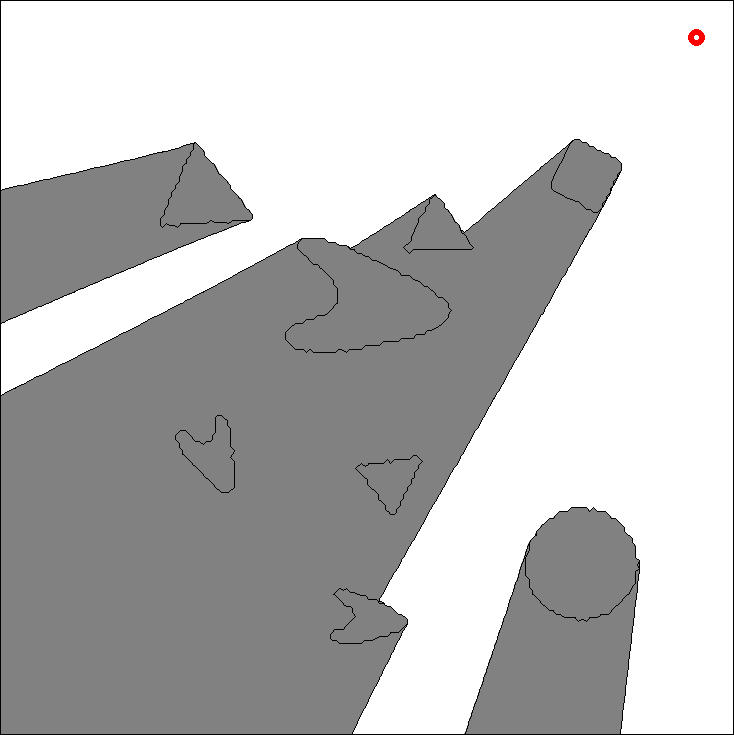
\includegraphics[width=2in]{media_exploration/2D_scene_01}
\end{tabular}
&\phantom{\parbox[t]{.5\textwidth}{
\begin{itemize}
 \item ``Frontier chasing''
 \item Heuristics
\end{itemize}}}
\end{tabular}
\end{tframe}

\addtocounter{framenumber}{-1}
\begin{tframe}{Autonomous Exploration}

\bigskip
\begin{tabular}{cl}
\begin{tabular}{c}
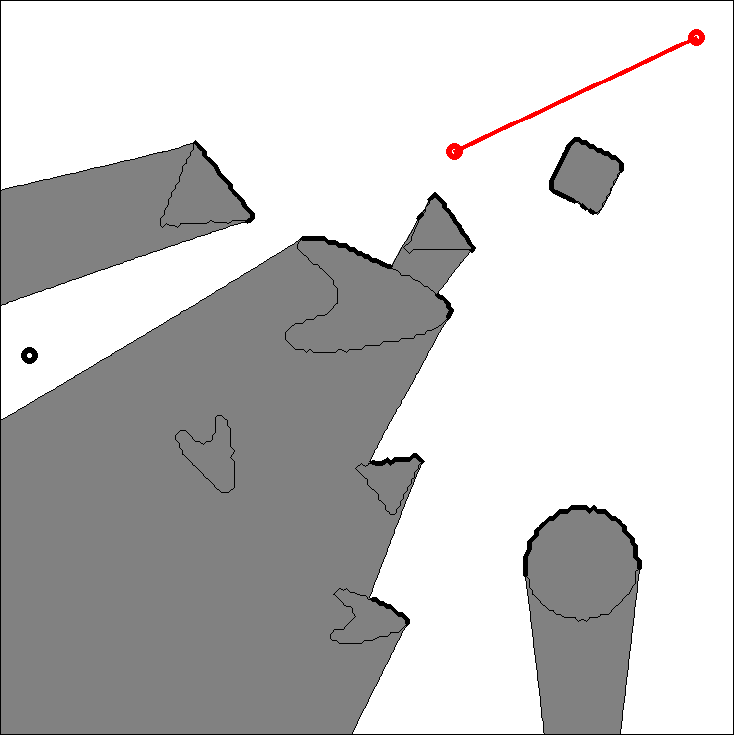
\includegraphics[width=2in]{media_exploration/2D_scene_02}
\end{tabular}
&\visible<2>{\parbox[t]{.5\textwidth}{
\begin{itemize}
 \item ``Frontier chasing''
 \item Heuristics
\end{itemize}}}
\end{tabular}
\end{tframe}


\begin{tframe}{Exploring a Random Room}
\begin{center}
\begin{tabular}{c}
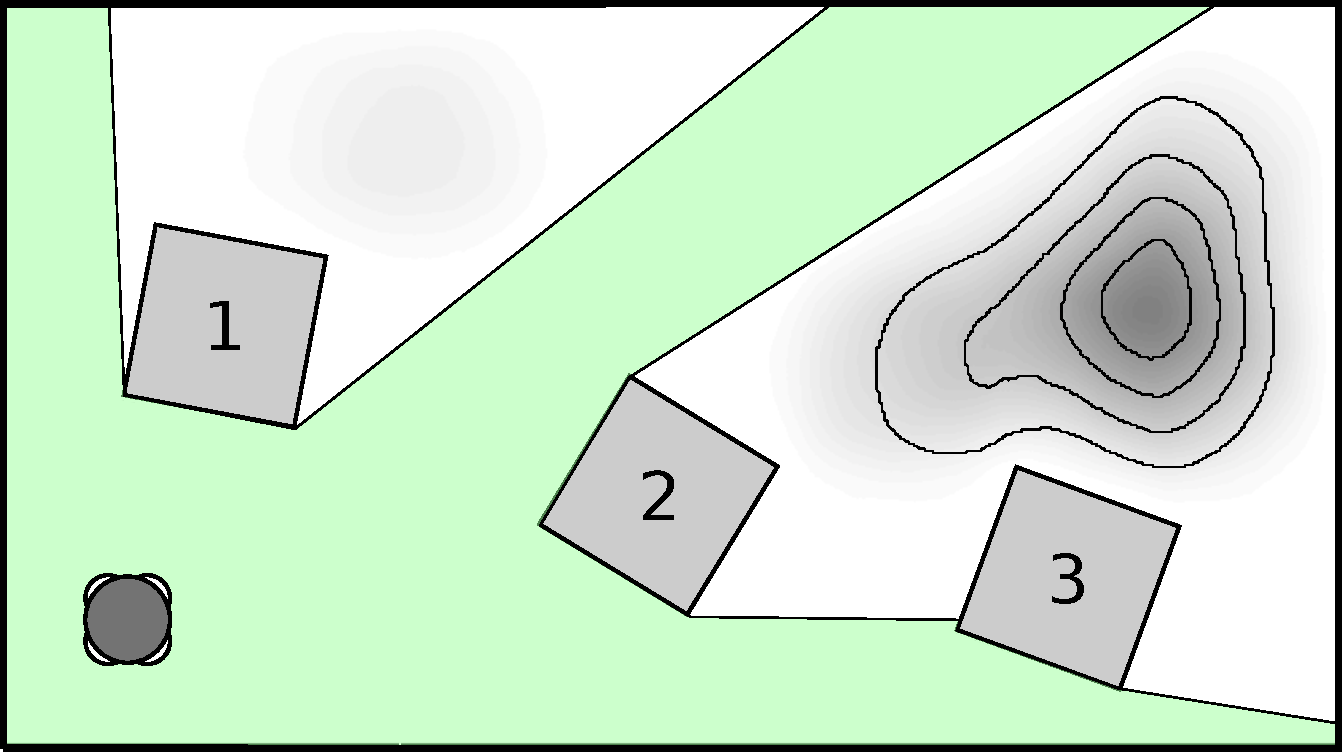
\includegraphics[height=1in]{media_exploration/random_block_marg}
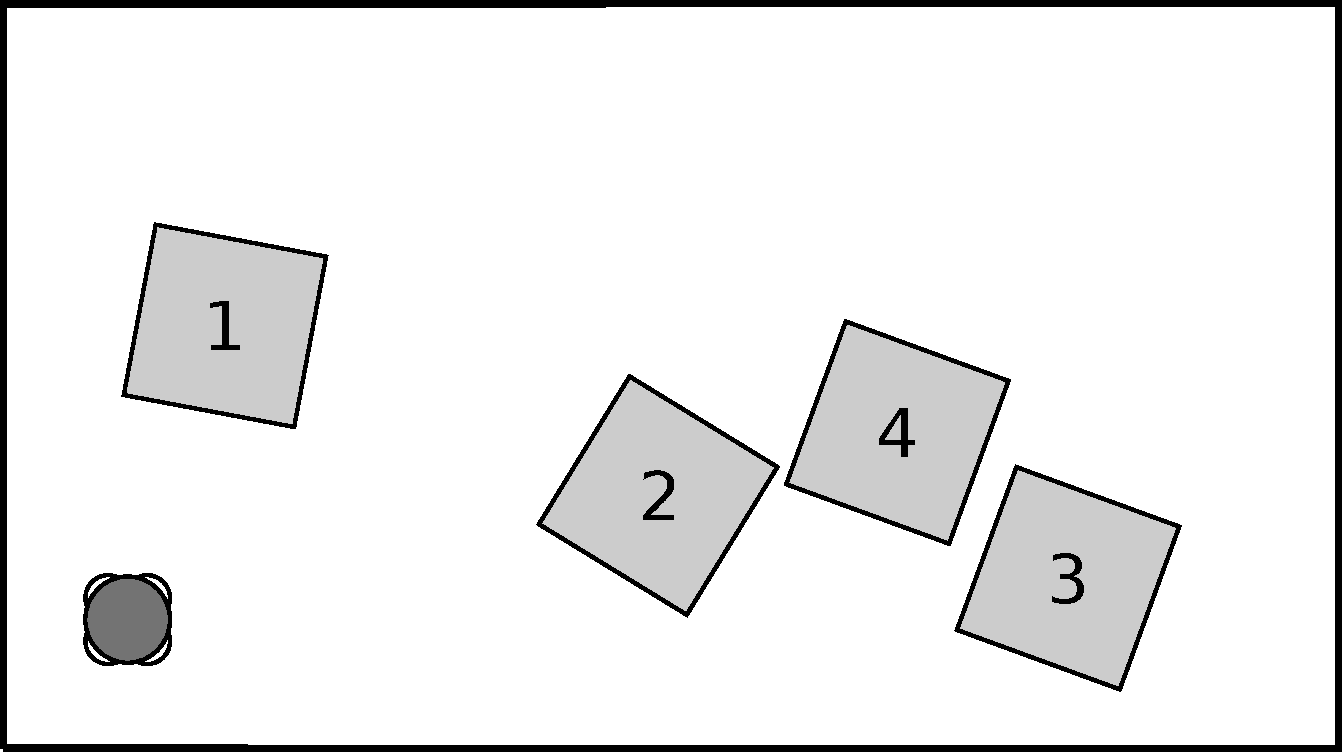
\includegraphics[height=1in]{media_exploration/random_block}
\end{tabular}
\end{center}
\begin{block}{}
 When features are coarse,
 the information content of an unmapped region is not
 always proportional to its size.  
\end{block}
\end{tframe}

\addtocounter{framenumber}{-1}
\begin{tframe}{Obstacle Density Determines Viewpoint}
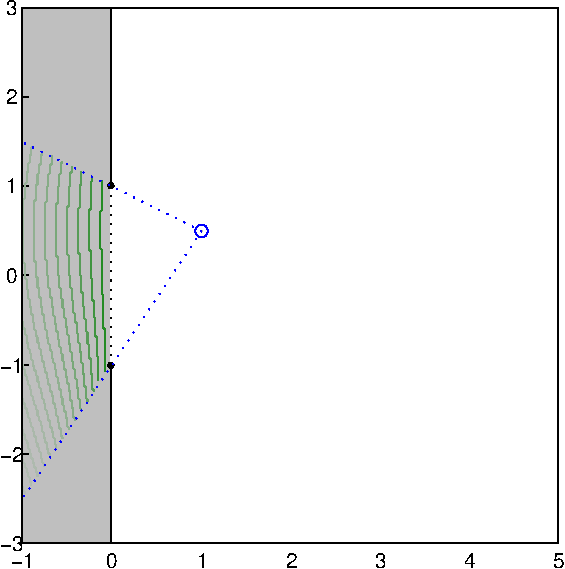
\includegraphics[width=2in]{media_exploration/penetration1}
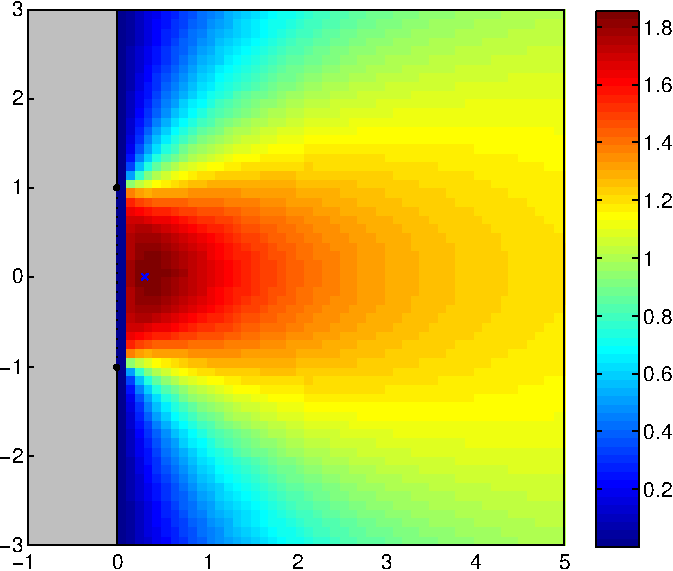
\includegraphics[width=2in]{media_exploration/JEnergy1}
\end{tframe}

\addtocounter{framenumber}{-1}
\begin{tframe}{Obstacle Density Determines Viewpoint}
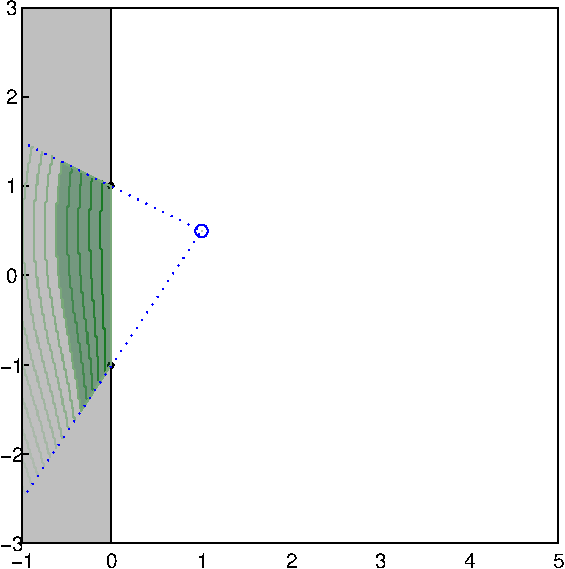
\includegraphics[width=2in]{media_exploration/penetration5}
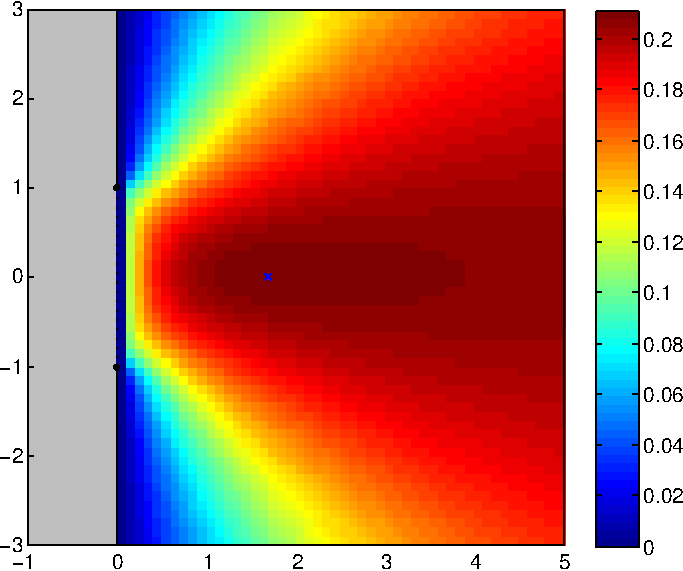
\includegraphics[width=2in]{media_exploration/JEnergy5}
\end{tframe}

\addtocounter{framenumber}{-1}
\begin{tframe}{Obstacle Density Determines Viewpoint}
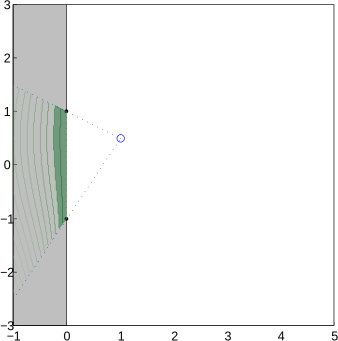
\includegraphics[width=2in]{media_exploration/penetration25}
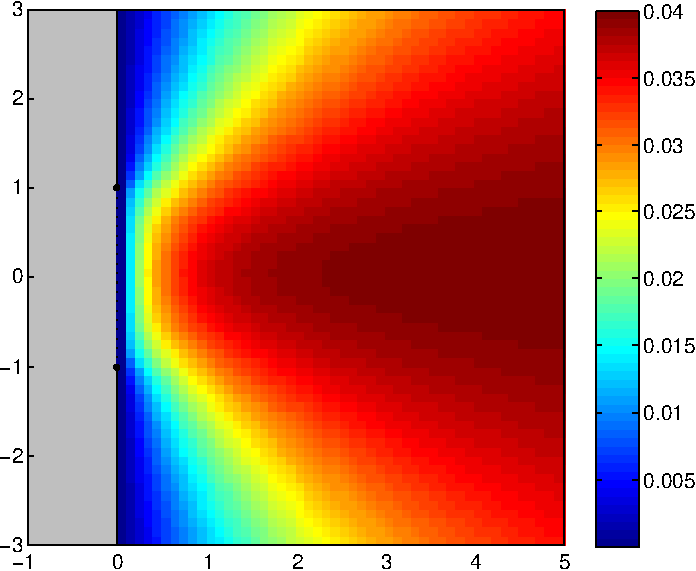
\includegraphics[width=2in]{media_exploration/JEnergy25}
\end{tframe}

\begin{tframe}{Ising-Type Obstacles}
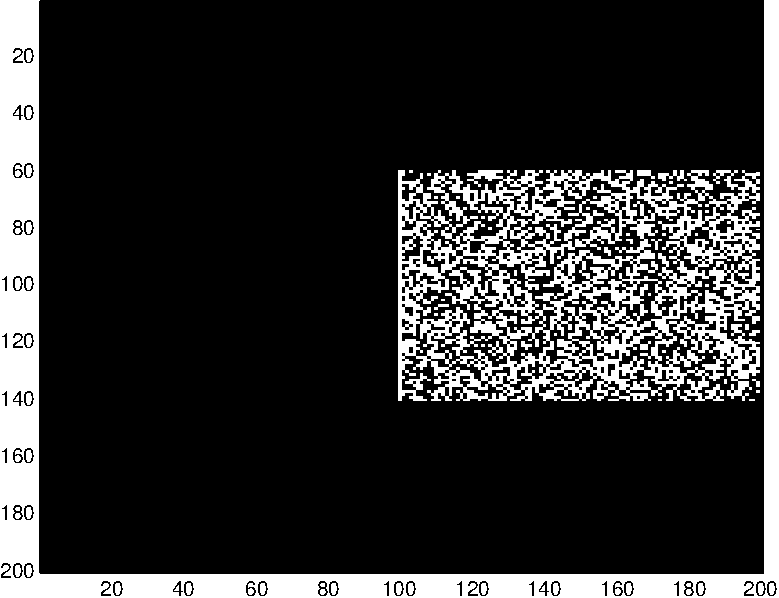
\includegraphics[width=2in]{media_exploration/ising000}
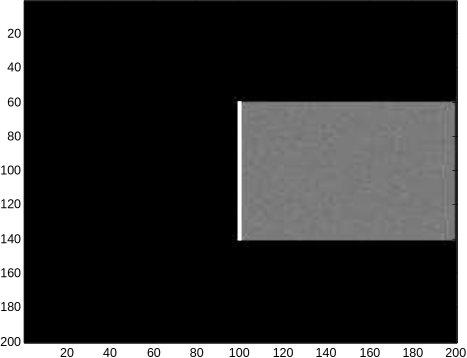
\includegraphics[width=2in]{media_exploration/marg000}

0 Iterations
\end{tframe}

\addtocounter{framenumber}{-1}
\begin{tframe}{Ising-Type Obstacles}
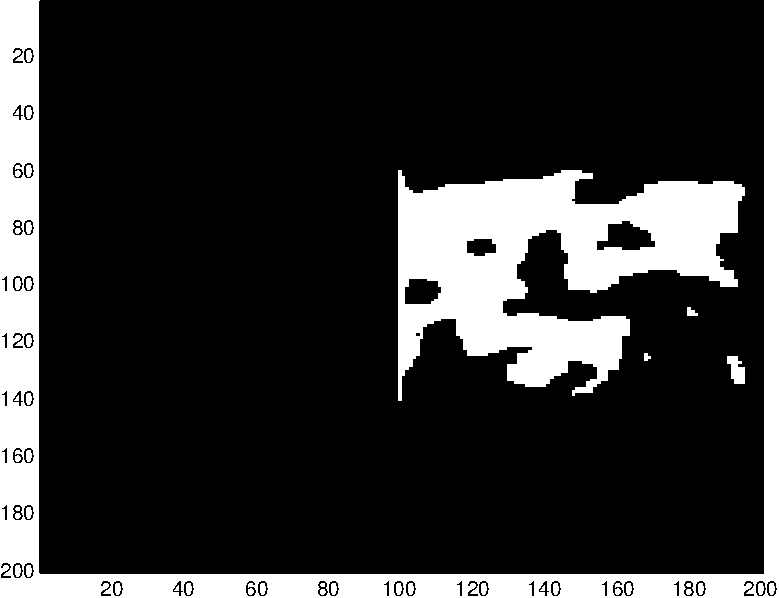
\includegraphics[width=2in]{media_exploration/ising025}
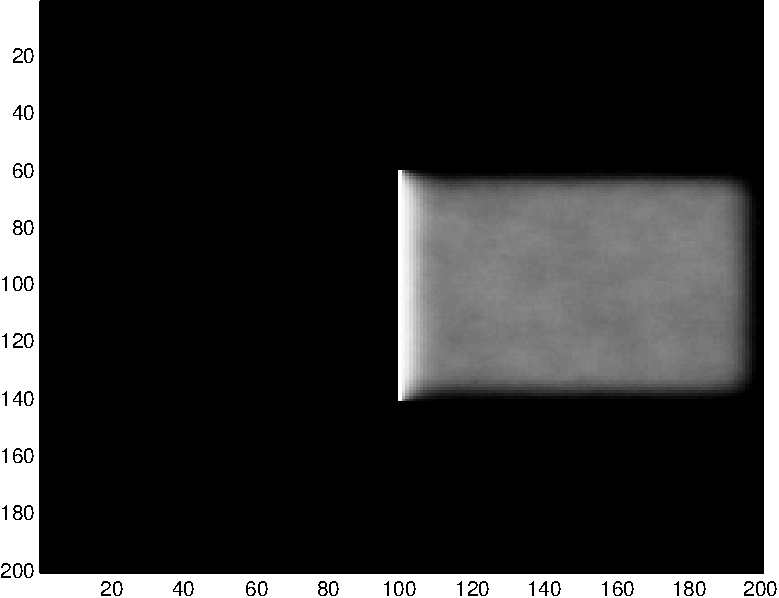
\includegraphics[width=2in]{media_exploration/marg025}

25 Iterations
\end{tframe}

\addtocounter{framenumber}{-1}
\begin{tframe}{Ising-Type Obstacles}
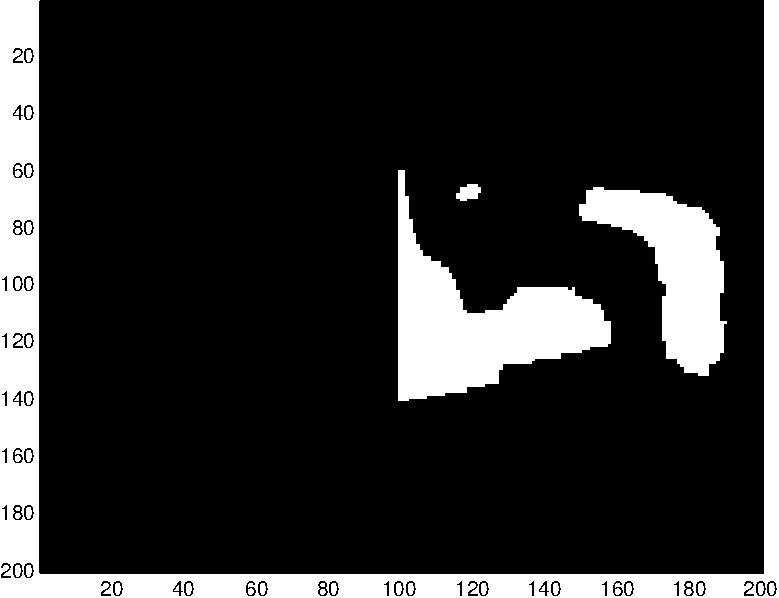
\includegraphics[width=2in]{media_exploration/ising100}
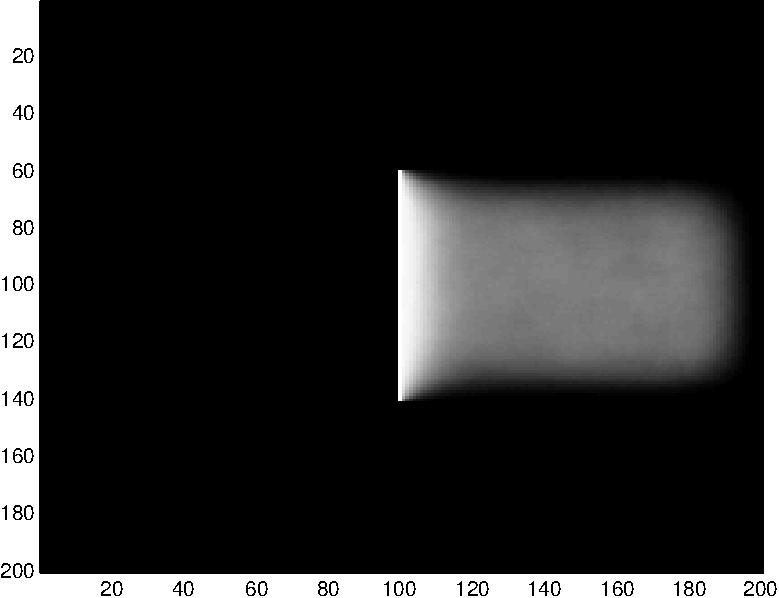
\includegraphics[width=2in]{media_exploration/marg100}

100 Iterations
\end{tframe}

\addtocounter{framenumber}{-1}
\begin{tframe}{Ising-Type Obstacles}
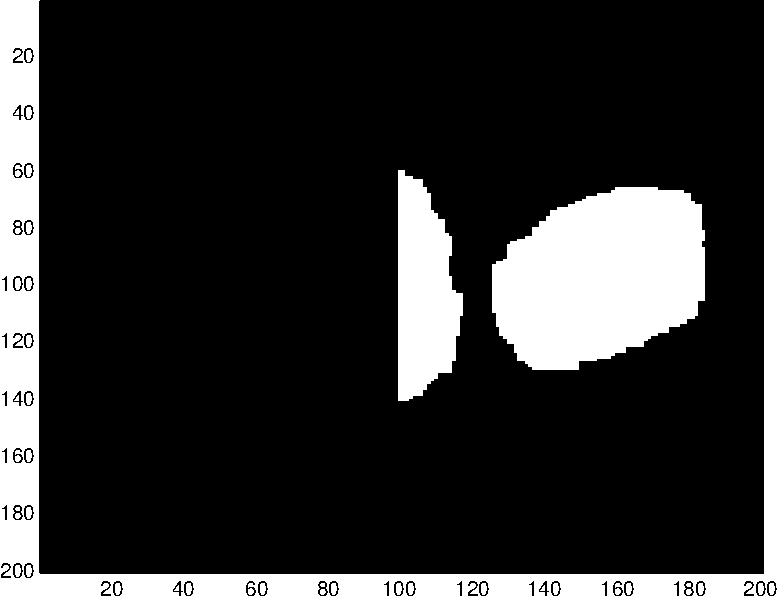
\includegraphics[width=2in]{media_exploration/ising225}
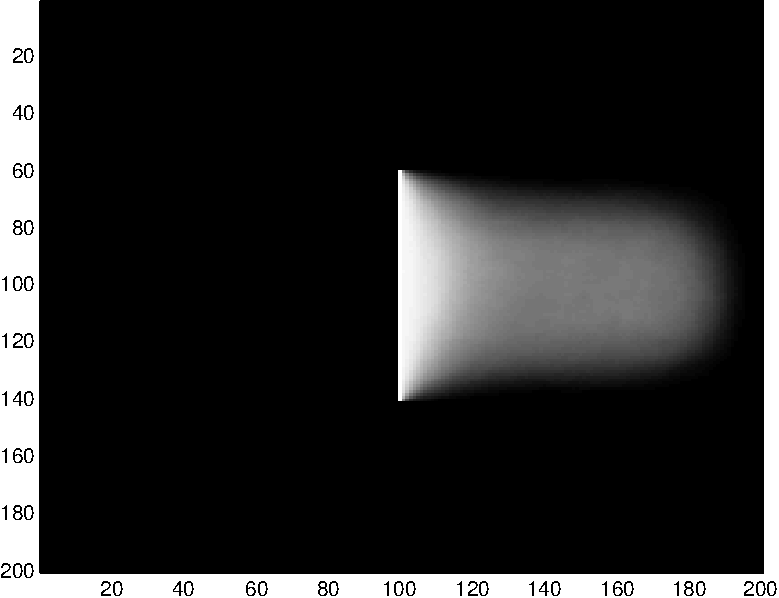
\includegraphics[width=2in]{media_exploration/marg225}

225 Iterations
\end{tframe}

\addtocounter{framenumber}{-1}
\begin{tframe}{Ising-Type Obstacles}
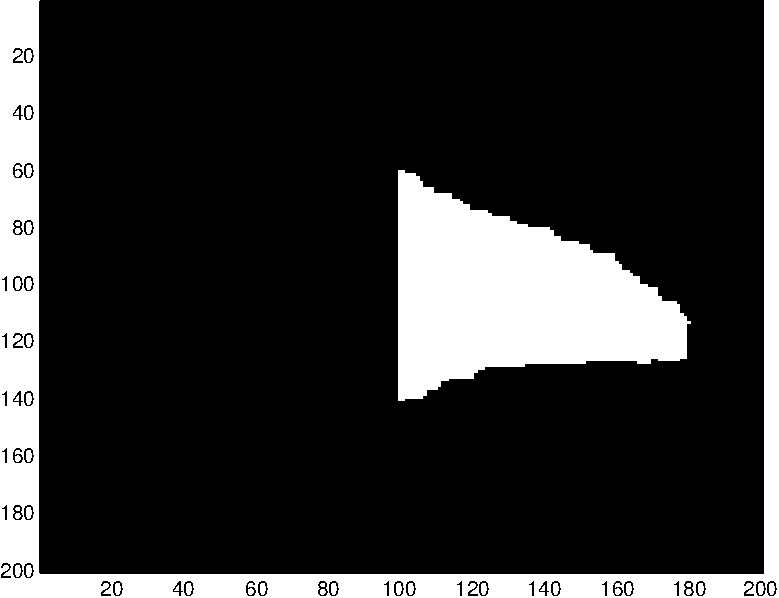
\includegraphics[width=2in]{media_exploration/ising400}
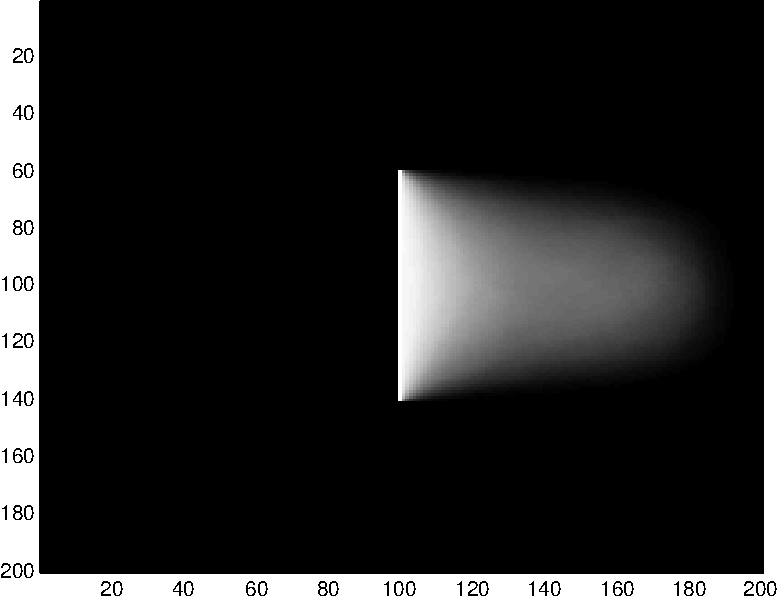
\includegraphics[width=2in]{media_exploration/marg400}

400 Iterations
\end{tframe}

\begin{tframe}{Ising-Type Penetration Profiles}

\bigskip
\begin{center}
\begin{tabular}{ccc}
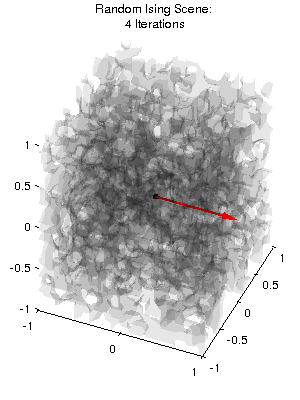
\includegraphics[height=1.2in]{media_exploration/ising_cell_004}&
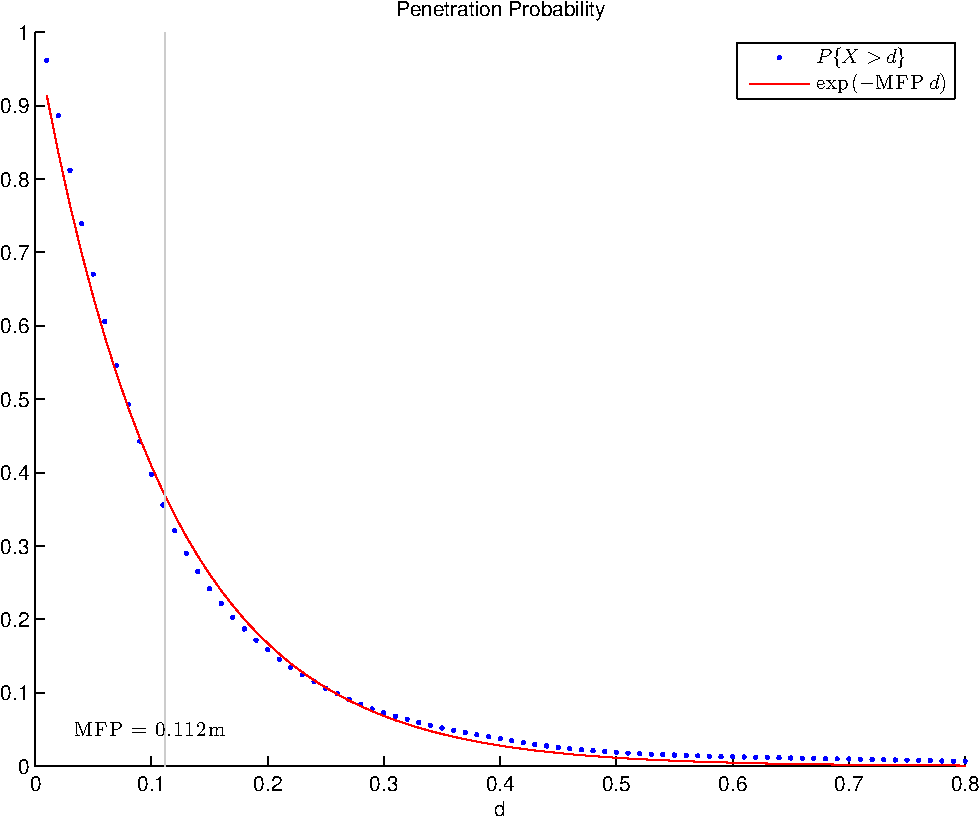
\includegraphics[height=1.2in]{media_exploration/ising_penetration_004}&
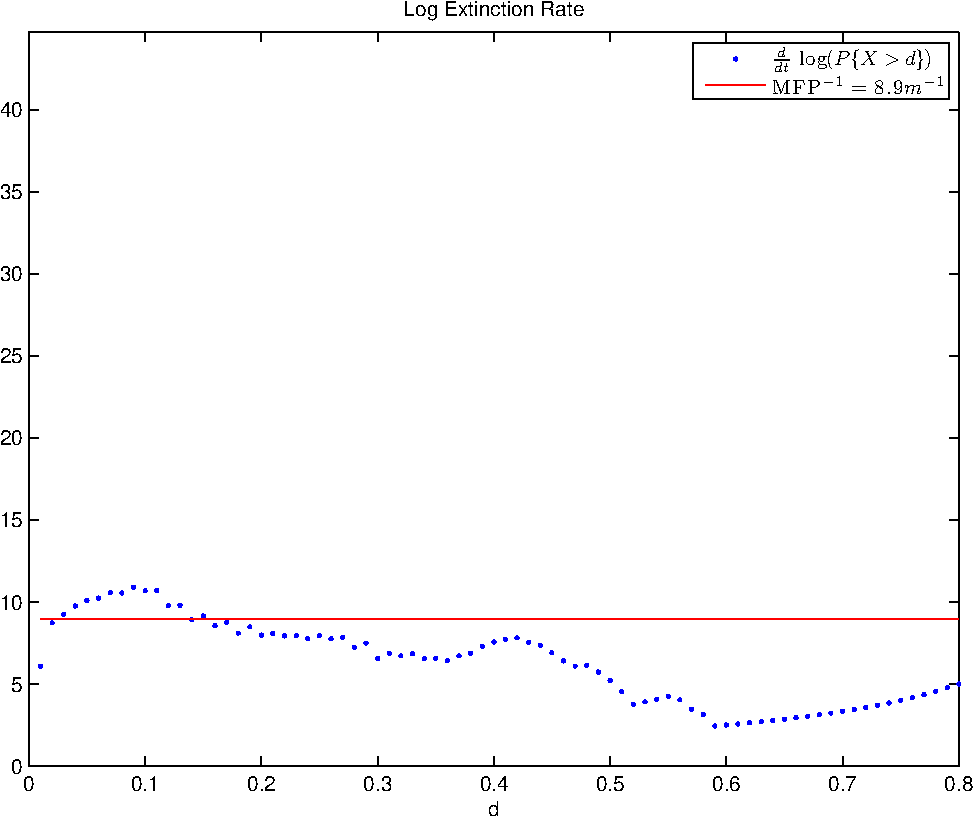
\includegraphics[height=1.2in]{media_exploration/ising_extinction_004}
\end{tabular}
 \end{center}

\bigskip
4 Iterations
\end{tframe}

\addtocounter{framenumber}{-1}
\begin{tframe}{Ising-Type Penetration Profiles}

\bigskip
\begin{center}
\begin{tabular}{ccc}
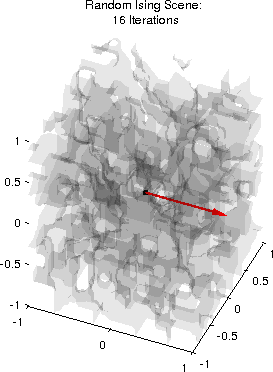
\includegraphics[height=1.2in]{media_exploration/ising_cell_016}&
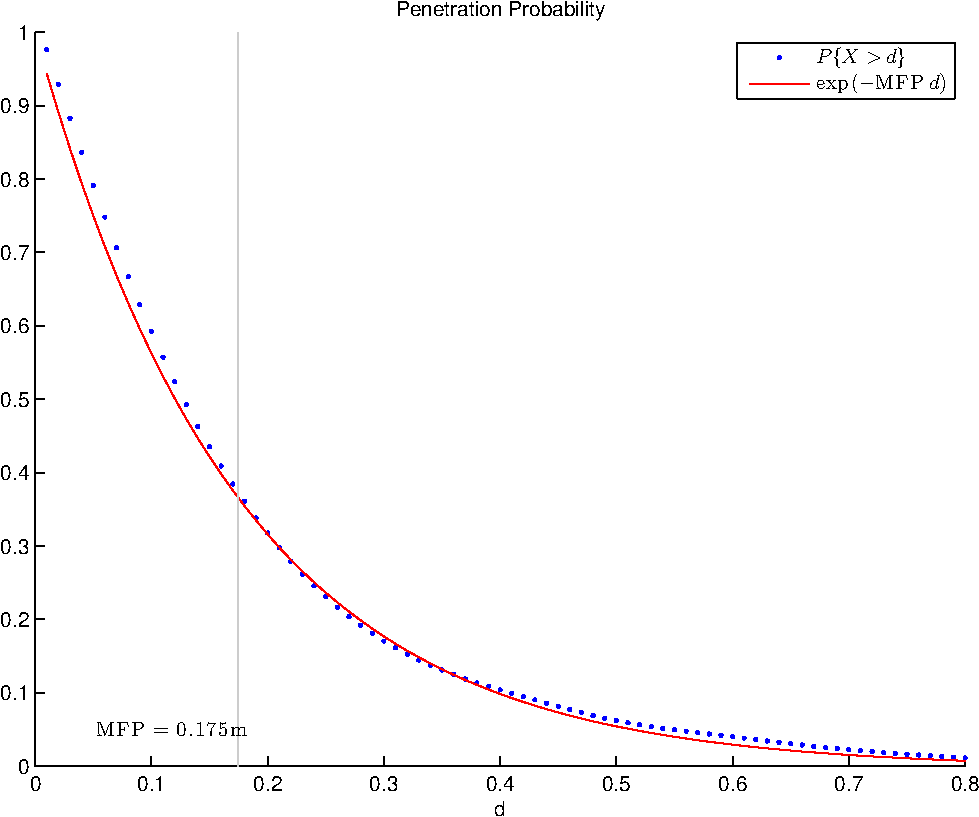
\includegraphics[height=1.2in]{media_exploration/ising_penetration_016}&
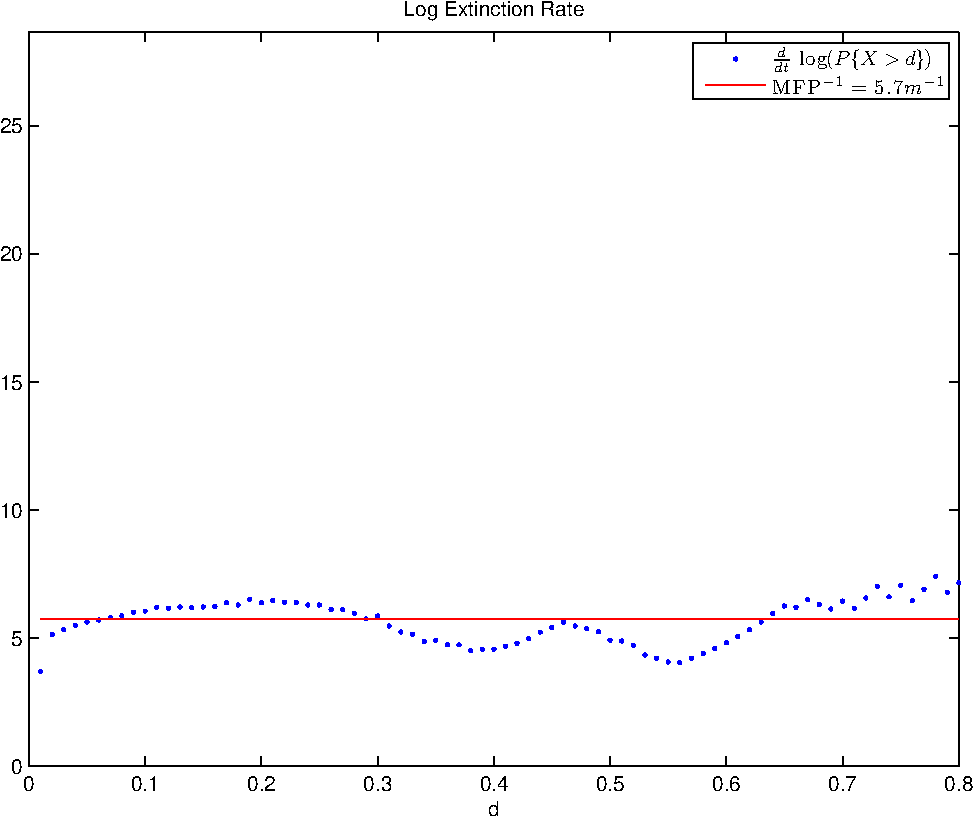
\includegraphics[height=1.2in]{media_exploration/ising_extinction_016}
\end{tabular}
 \end{center}

\bigskip
16 Iterations
\end{tframe}

\addtocounter{framenumber}{-1}
\begin{tframe}{Ising-Type Penetration Profiles}

\bigskip
\begin{center}
\begin{tabular}{ccc}
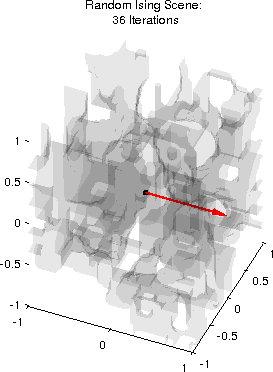
\includegraphics[height=1.2in]{media_exploration/ising_cell_036}&
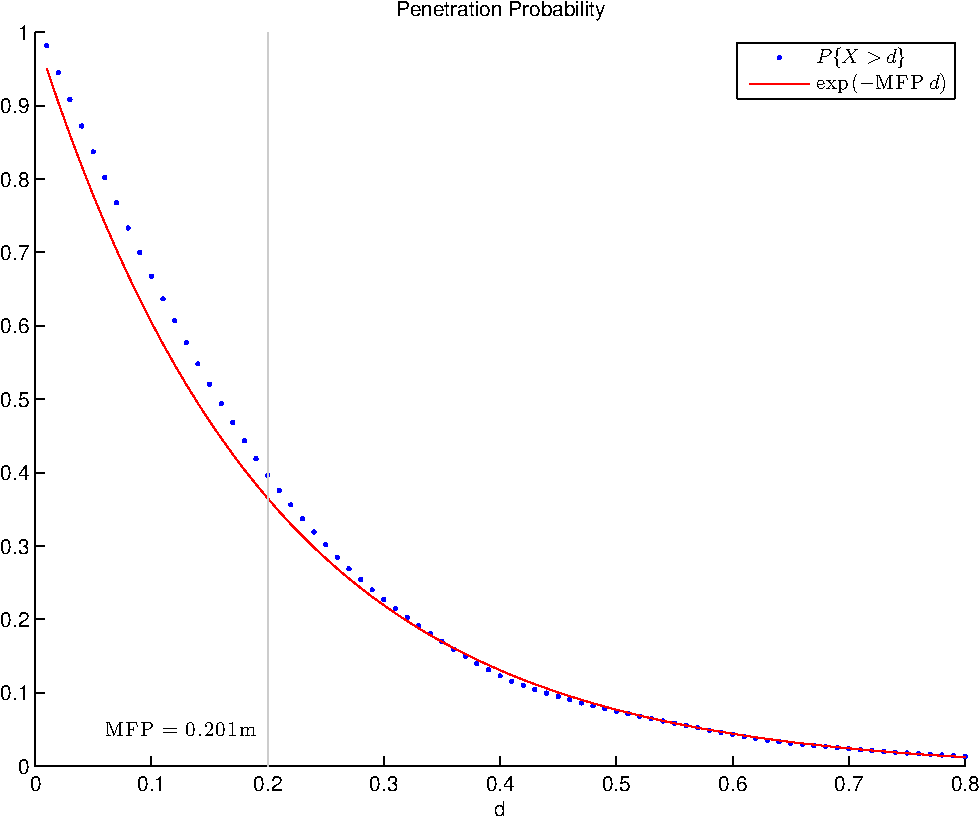
\includegraphics[height=1.2in]{media_exploration/ising_penetration_036}&
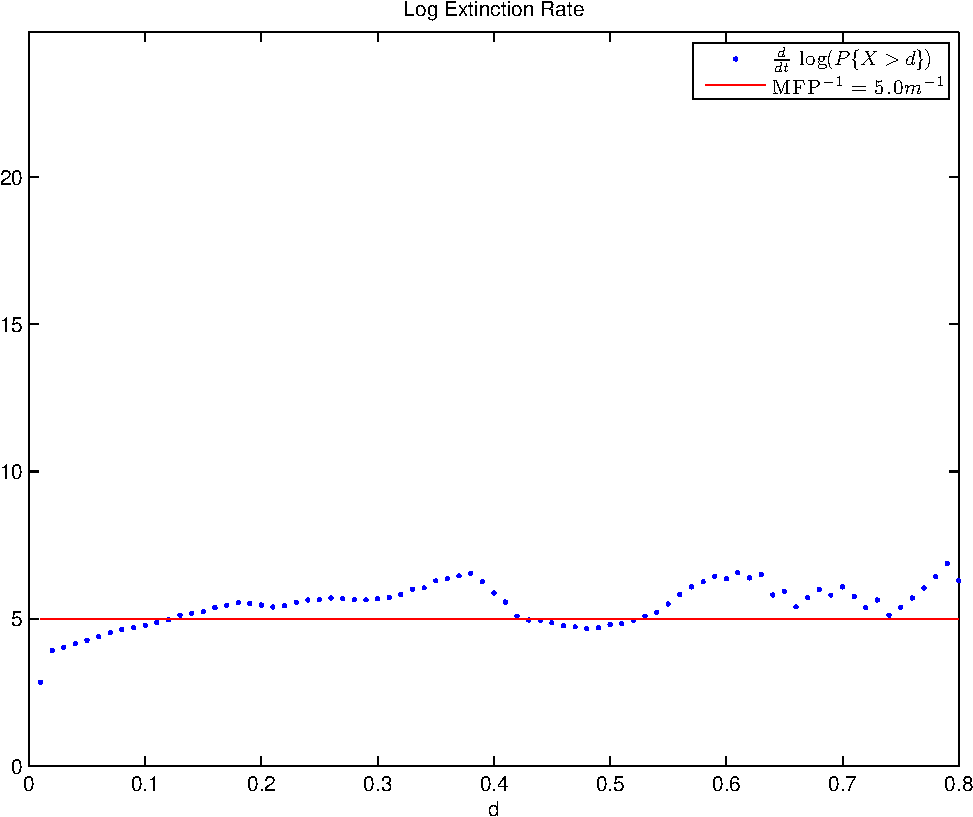
\includegraphics[height=1.2in]{media_exploration/ising_extinction_036}
\end{tabular}
 \end{center}

\bigskip
36 Iterations
\end{tframe}

\begin{tframe}{Ising-Type Penetration Profiles}

\bigskip
\begin{center}
\begin{tabular}{ccc}
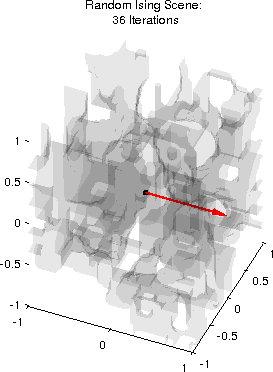
\includegraphics[height=1.2in]{media_exploration/ising_cell_036}&
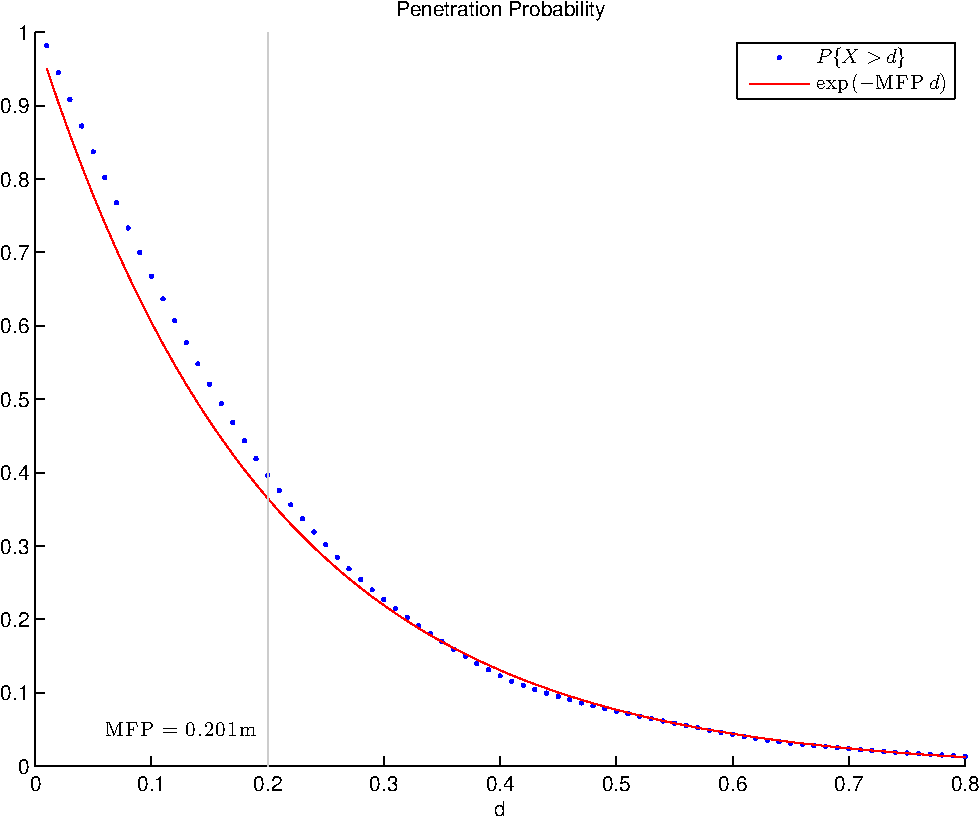
\includegraphics[height=1.2in]{media_exploration/ising_penetration_036}&
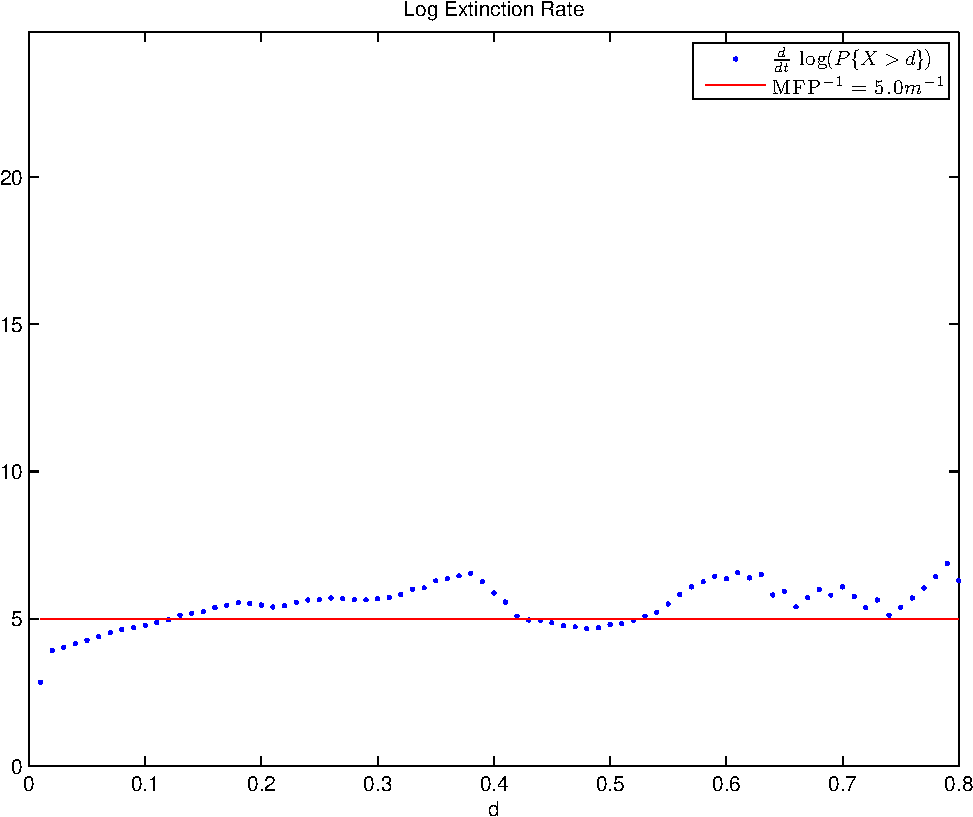
\includegraphics[height=1.2in]{media_exploration/ising_extinction_036}
\end{tabular}
 \end{center}

\bigskip
36 Iterations
\end{tframe}

\begin{tframe}{Information-Seeking Control}

\bigskip
\begin{center}
\begin{tabular}{cc}
\begin{tabular}{c}
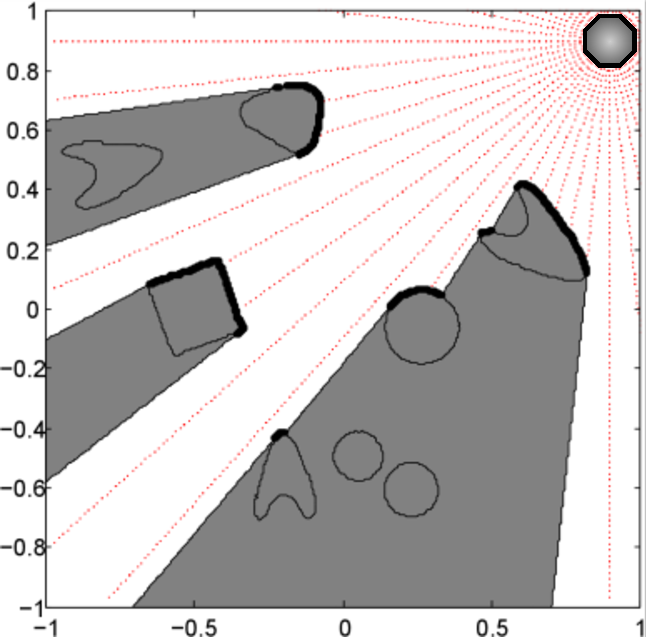
\includegraphics[height=2in]{media_exploration/first_view}
\end{tabular}
&
\parbox[t]{.5\textwidth}{
The information value of a new viewpoint is equal to the uncertainty of
the measurement to be taken there.
}
\end{tabular}
 \end{center}
\end{tframe}

\addtocounter{framenumber}{-1}
\begin{tframe}{Information-Seeking Control}

\bigskip
\begin{center}
\begin{tabular}{cc}
\begin{tabular}{c}
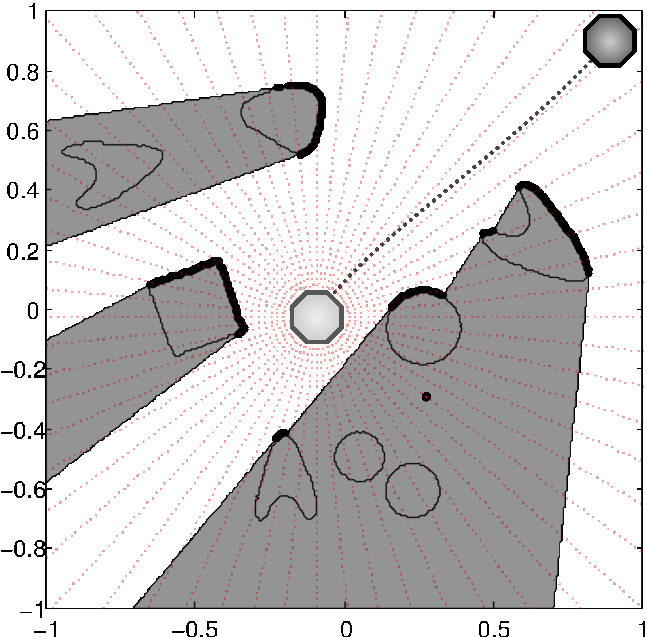
\includegraphics[height=2in]{media_exploration/first_hypoth}
\end{tabular}
&
\parbox[t]{.5\textwidth}{
The information value of a new viewpoint is equal to the uncertainty of
the measurement to be taken there.
}
\end{tabular}
 \end{center}
\end{tframe}

\addtocounter{framenumber}{-1}
\begin{tframe}{Information-Seeking Control}

\bigskip
\begin{center}
\begin{tabular}{cc}
\begin{tabular}{c}
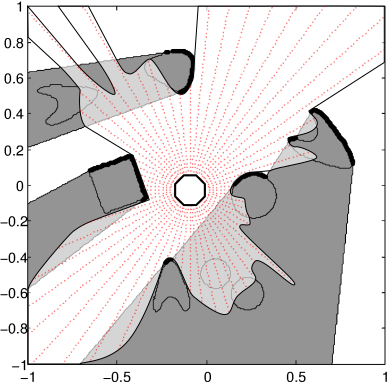
\includegraphics[height=2in]{media_exploration/first_meas}
\end{tabular}
&
\parbox[t]{.5\textwidth}{
The information value of a new viewpoint is equal to the uncertainty of
the measurement to be taken there.
}
\end{tabular}
 \end{center}
\end{tframe}

\begin{tframe}{View Value}
\begin{center}
\begin{align*}
E_t(x) \approx \sum_{ij}& 
\underset{\text{Marginal value of revealing point at $x+g_{ij}$}}
{\underbrace{w_i H(\PP_t[x+g_{ij}\in\A])}}\\
&\qquad\cdot\,
\underset{\text{Probability of revealing point at $x+g_{ij}$}}
{\underbrace{\prod_{i\1<i}\PP_t[x+g_{i\1j}\in\A]^{s/\operatorname{MFP}(x+g_{i\1j})}}}
\end{align*}
where $H(p) = -p\log p - (1-p)\log(1-p)$.
\end{center}
\end{tframe}

\begin{tframe}{Poisson-Voronoi Proxy}
\bigskip
\begin{tabular}{ccc}
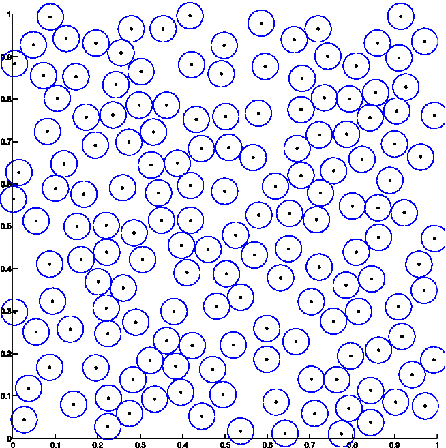
\includegraphics[height=1.2in]{media_exploration/poisson_disk}&
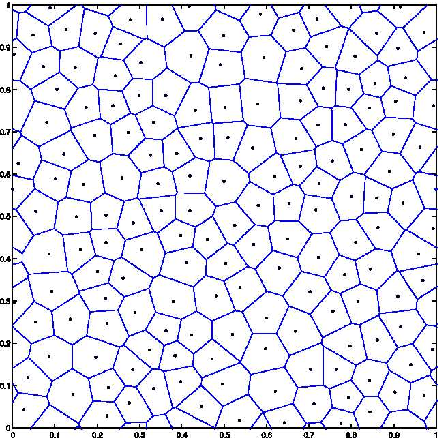
\includegraphics[height=1.1in]{media_exploration/voronoi}&
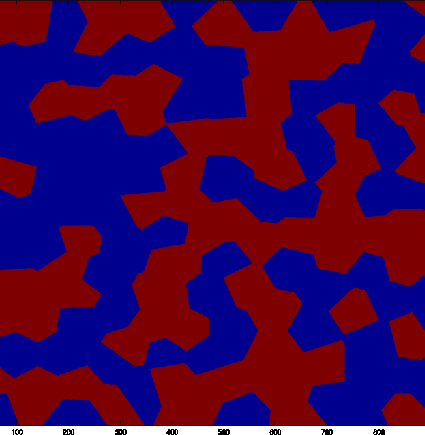
\includegraphics[height=1.3in]{media_exploration/voronoi_chex}\\
Poisson-Disk Sampling &
Voronoi Tesselation &
Voronoi Checkerboard
\end{tabular}
\end{tframe}

\begin{tframe}{Poisson-Voronoi Proxy}
\begin{center}
\begin{tabular}{c}
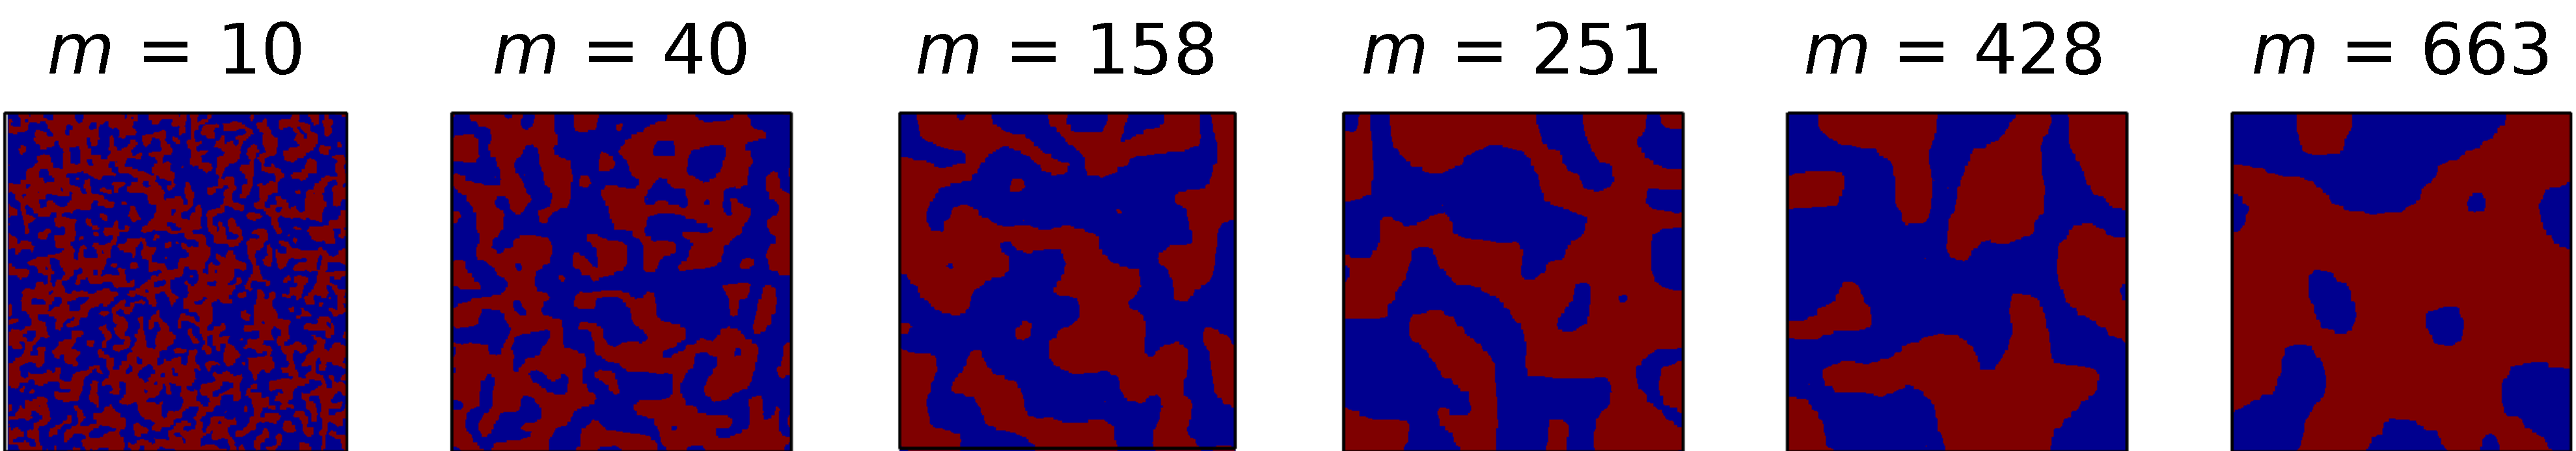
\includegraphics[width=4in]{media_exploration/entropy_ising}\\
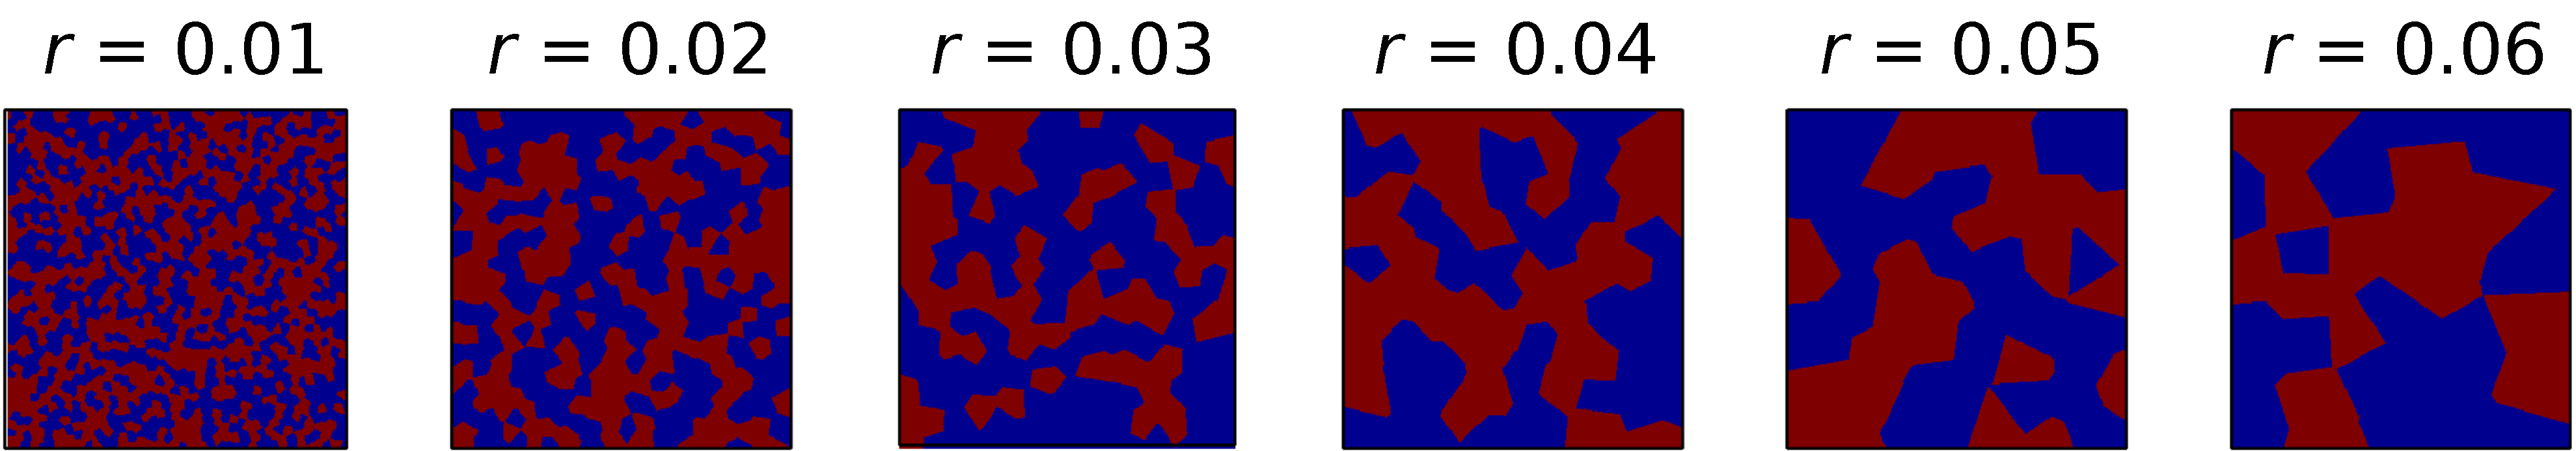
\includegraphics[width=4in]{media_exploration/entropy_chex}
\end{tabular}
\end{center}
\end{tframe}

\begin{tframe}{Poisson-Voronoi Proxy}

\bigskip
\begin{tabular}{ccc}
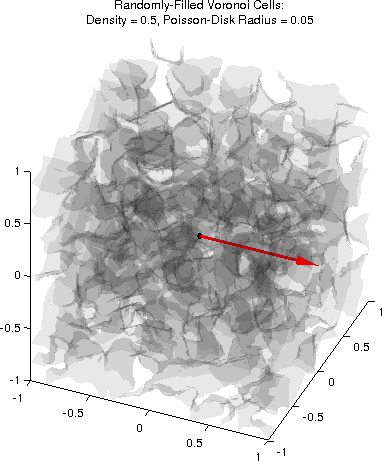
\includegraphics[height=1.2in]{media_exploration/cell_05}&
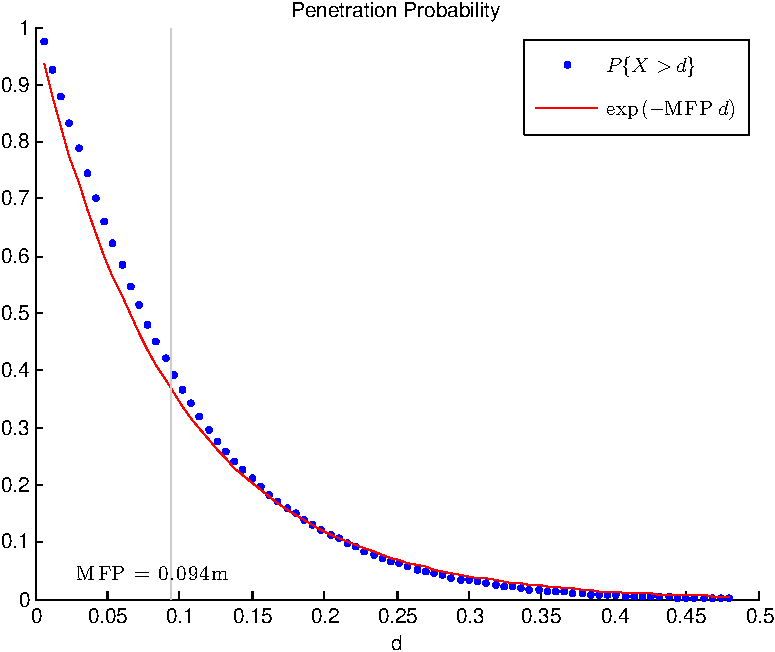
\includegraphics[height=1.2in]{media_exploration/penetration_05}&
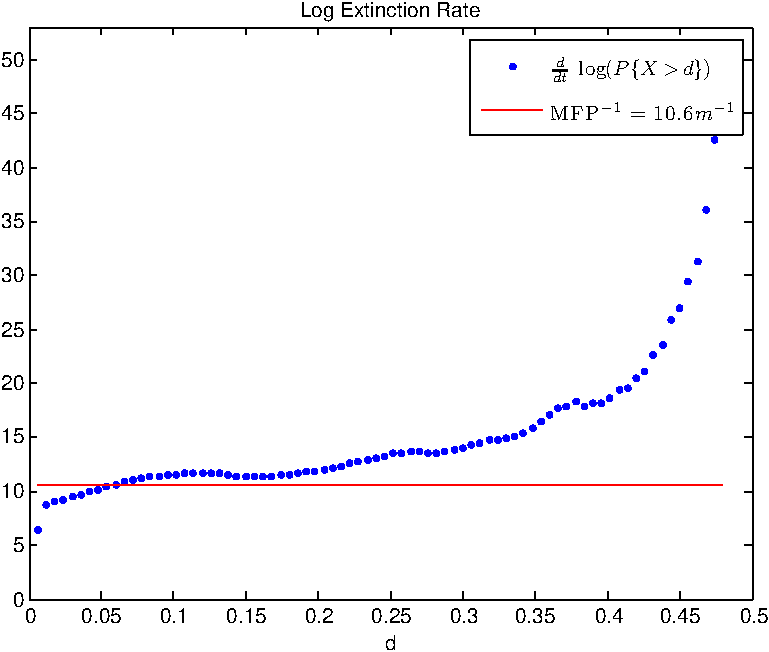
\includegraphics[height=1.2in]{media_exploration/extinction_05}
\end{tabular}

Mean free path scales directly with Poisson-disc radius,
so this needs to be computed only once
\end{tframe}


\begin{tframe}{Computing Graph Weights $w_i$}

\bigskip
\begin{center}
\begin{tabular}{cc}
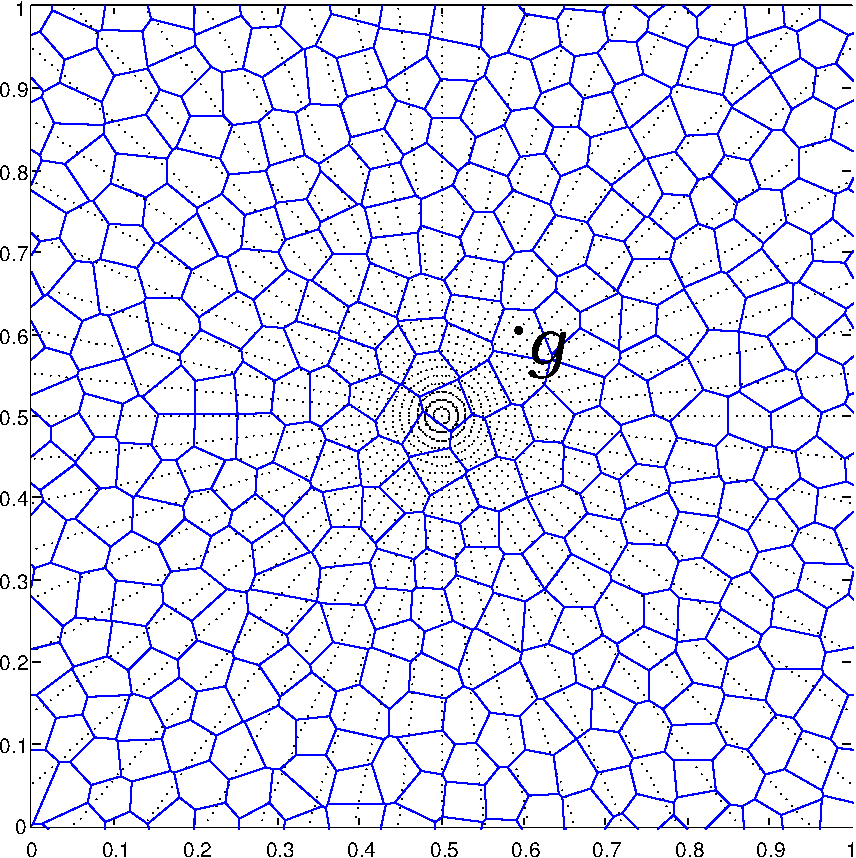
\includegraphics[height=1.5in]{media_exploration/voronoi_grid}&
\phantom{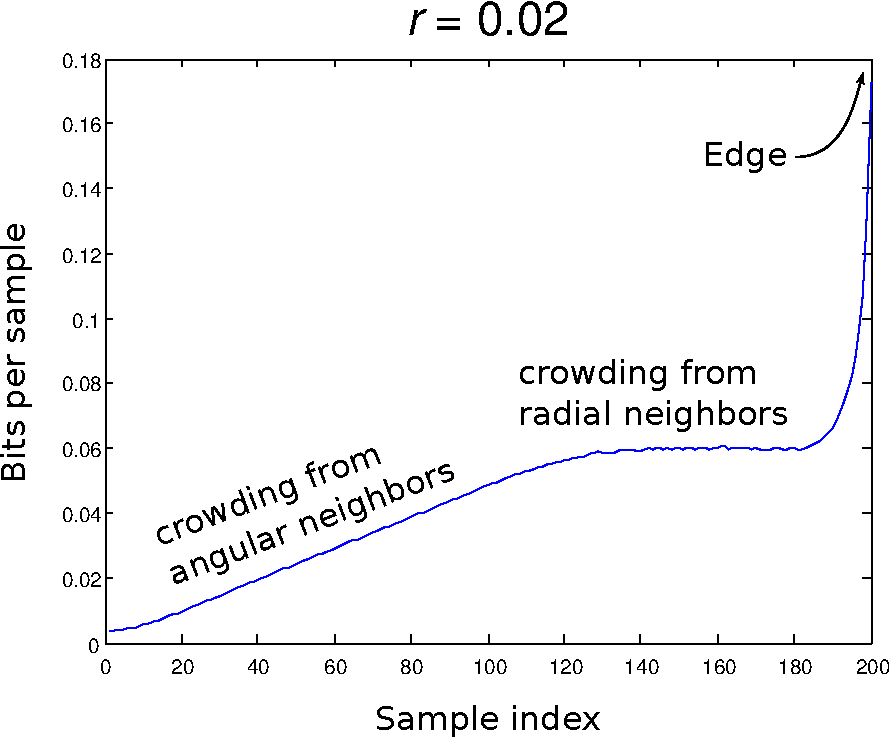
\includegraphics[height=1.5in]{media_exploration/weight_profile}}
\end{tabular}
\end{center}
\end{tframe}

\addtocounter{framenumber}{-1}
\begin{tframe}{Computing Graph Weights $w_i$}

\bigskip
\begin{center}
\begin{tabular}{cc}
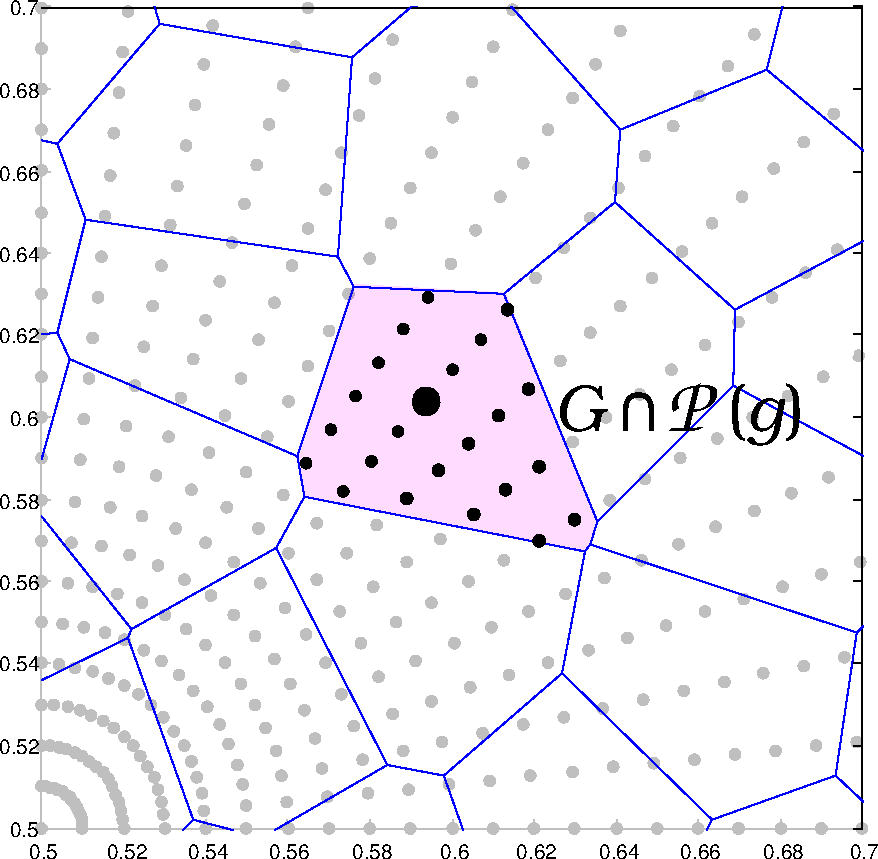
\includegraphics[height=1.5in]{media_exploration/voronoi_grid_closeup}&
\visible<2>{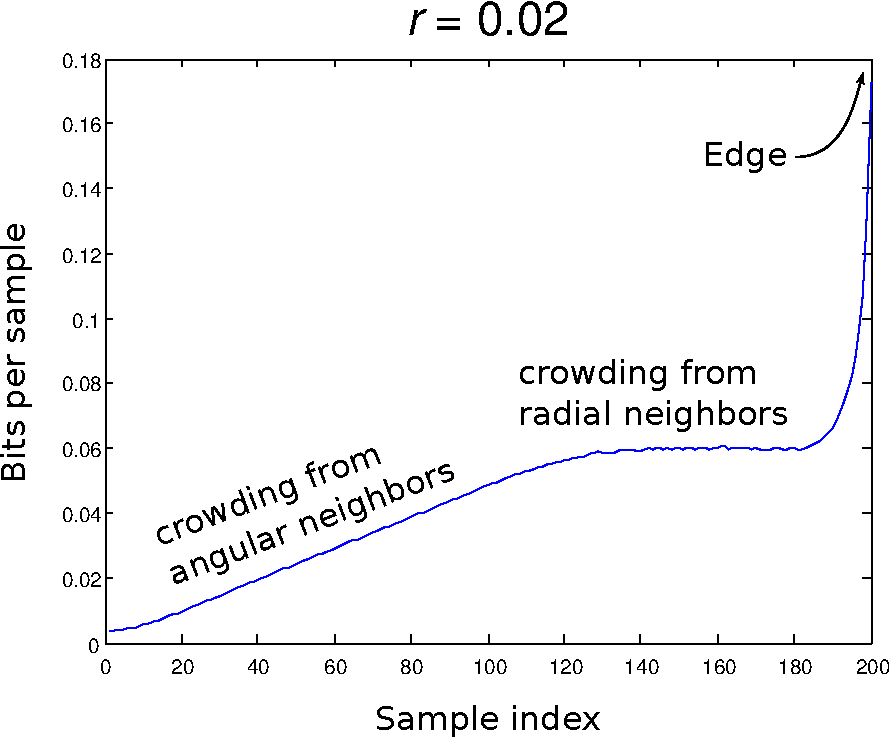
\includegraphics[height=1.5in]{media_exploration/weight_profile}}
\end{tabular}
\end{center}
\end{tframe}

\begin{tframe}{Computing Graph Weights $w_i$}

\bigskip
\begin{center}
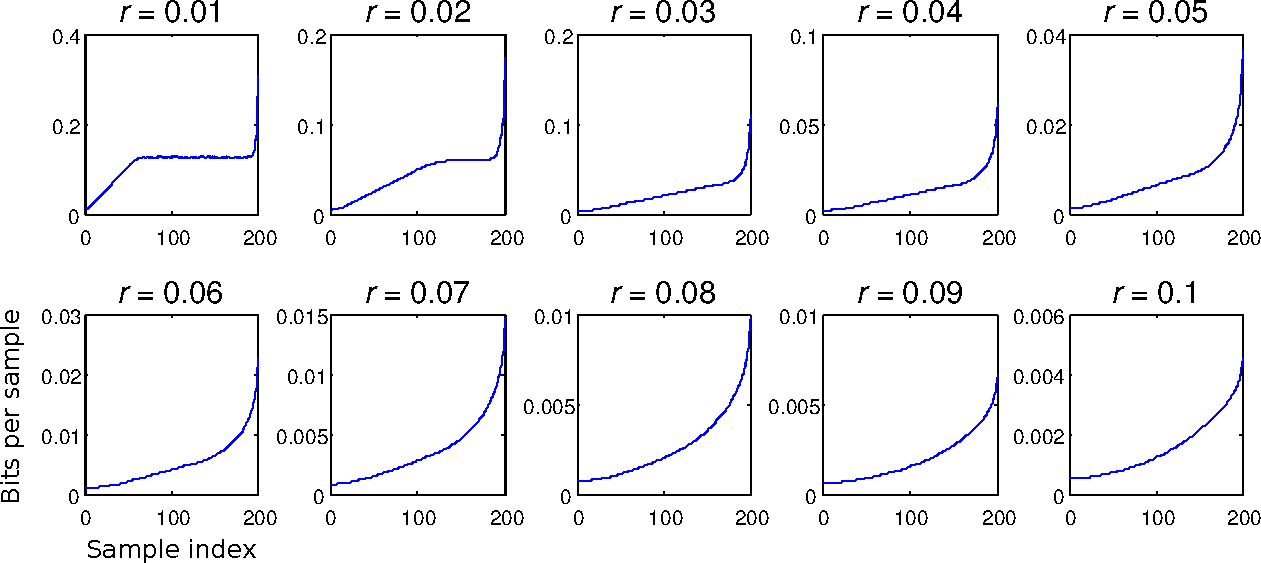
\includegraphics[width=4in]{media_exploration/weight_profiles}
\end{center}
\end{tframe}

\begin{tframe}{3D Graph Weights}
\begin{center}
\begin{tabular}{cc}
\begin{tabular}{c}
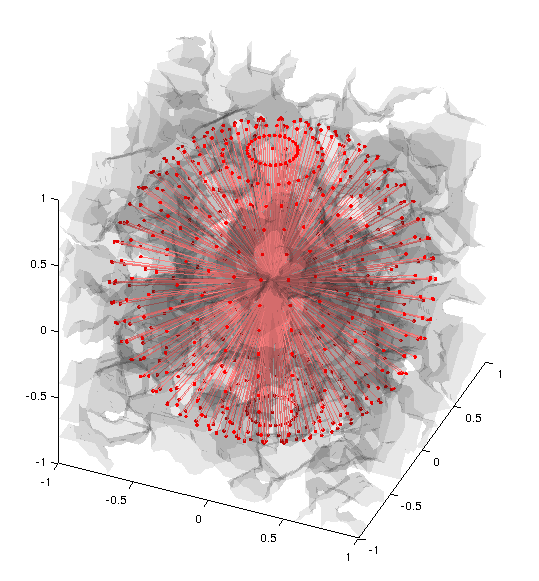
\includegraphics[height=1.5in]{media_exploration/samples.png}
\end{tabular}&
\begin{tabular}{cc}
\includegraphics[width=1in]{media_exploration/W02}&
\includegraphics[width=1in]{media_exploration/W04}\\
\includegraphics[width=1in]{media_exploration/W06}&
\includegraphics[width=1in]{media_exploration/W08}
\end{tabular}
\end{tabular}
\end{center}
\end{tframe}

\begin{tframe}{2D Exploration}
\begin{center}

\bigskip
\begin{tabular}{ccc}
\includegraphics[width=1.2in]{media_exploration/2D_scene_01}&
\includegraphics[width=1.2in]{media_exploration/2D_marginal_01}&
\includegraphics[width=1.2in]{media_exploration/2D_energy_01}
\\ Visibility & Marginals & View Value
\end{tabular}
\end{center}
\end{tframe}

\addtocounter{framenumber}{-1}
\begin{tframe}{2D Exploration}
\begin{center}

\bigskip
\begin{tabular}{ccc}
\includegraphics[width=1.2in]{media_exploration/2D_scene_02}&
\includegraphics[width=1.2in]{media_exploration/2D_marginal_02}&
\includegraphics[width=1.2in]{media_exploration/2D_energy_02}
\\ Visibility & Marginals & View Value
\end{tabular}
\end{center}
\end{tframe}

\addtocounter{framenumber}{-1}
\begin{tframe}{2D Exploration}
\begin{center}

\bigskip
\begin{tabular}{ccc}
\includegraphics[width=1.2in]{media_exploration/2D_scene_03}&
\includegraphics[width=1.2in]{media_exploration/2D_marginal_03}&
\includegraphics[width=1.2in]{media_exploration/2D_energy_03}
\\ Visibility & Marginals & View Value
\end{tabular}
\end{center}
\end{tframe}

\addtocounter{framenumber}{-1}
\begin{tframe}{2D Exploration}
\begin{center}

\bigskip
\begin{tabular}{ccc}
\includegraphics[width=1.2in]{media_exploration/2D_scene_04}&
\includegraphics[width=1.2in]{media_exploration/2D_marginal_04}&
\includegraphics[width=1.2in]{media_exploration/2D_energy_04}
\\ Visibility & Marginals & View Value
\end{tabular}
\end{center}
\end{tframe}

\addtocounter{framenumber}{-1}
\begin{tframe}{2D Exploration}
\begin{center}

\bigskip
\begin{tabular}{ccc}
\includegraphics[width=1.2in]{media_exploration/2D_scene_05}&
\includegraphics[width=1.2in]{media_exploration/2D_marginal_05}&
\includegraphics[width=1.2in]{media_exploration/2D_energy_05}
\\ Visibility & Marginals & View Value
\end{tabular}
\end{center}
\end{tframe}

\begin{tframe}{3D Exploration}
\begin{center}

\bigskip
\begin{tabular}{ccc}
\includegraphics[width=1.2in]{media_exploration/view_01}&
\includegraphics[width=1.2in]{media_exploration/marginal_01}&
\includegraphics[width=1.2in]{media_exploration/energy_01}
\\ Visibility & Marginals & View Value
\end{tabular}
\end{center}
\end{tframe}

\addtocounter{framenumber}{-1}
\begin{tframe}{3D Exploration}
\begin{center}

\bigskip
\begin{tabular}{ccc}
\includegraphics[width=1.2in]{media_exploration/view_02}&
\includegraphics[width=1.2in]{media_exploration/marginal_02}&
\includegraphics[width=1.2in]{media_exploration/energy_02}
\\ Visibility & Marginals & View Value
\end{tabular}
\end{center}
\end{tframe}

\addtocounter{framenumber}{-1}
\begin{tframe}{3D Exploration}
\begin{center}

\bigskip
\begin{tabular}{ccc}
\includegraphics[width=1.2in]{media_exploration/view_03}&
\includegraphics[width=1.2in]{media_exploration/marginal_03}&
\includegraphics[width=1.2in]{media_exploration/energy_03}
\\ Visibility & Marginals & View Value
\end{tabular}
\end{center}
\end{tframe}

\addtocounter{framenumber}{-1}
\begin{tframe}{3D Exploration}
\begin{center}

\bigskip
\begin{tabular}{ccc}
\includegraphics[width=1.2in]{media_exploration/view_04}&
\includegraphics[width=1.2in]{media_exploration/marginal_04}&
\includegraphics[width=1.2in]{media_exploration/energy_04}
\\ Visibility & Marginals & View Value
\end{tabular}
\end{center}
\end{tframe}

\addtocounter{framenumber}{-1}
\begin{tframe}{3D Exploration}
\begin{center}

\bigskip
\begin{tabular}{ccc}
\includegraphics[width=1.2in]{media_exploration/view_05}&
\includegraphics[width=1.2in]{media_exploration/marginal_05}&
\includegraphics[width=1.2in]{media_exploration/energy_05}
\\ Visibility & Marginals & View Value
\end{tabular}
\end{center}
\end{tframe}

\begin{tframe}{Comparisons}
\begin{center}
\begin{tabular}{c}
\includegraphics[width=4in]{media_exploration/simple_cropped}\\
\includegraphics[width=4in]{media_exploration/ising_cropped}
\end{tabular}
\end{center}
\end{tframe}

\begin{tframe}{Speedup: Parallel Bits}

\bigskip
\begin{center}
\begin{tabular}{cc}
\includegraphics[height=1.4in]{media_exploration/iso-01}&
\includegraphics[height=1.4in]{media_exploration/par000}
\end{tabular}
\end{center}
\end{tframe}

\addtocounter{framenumber}{-1}
\begin{tframe}{Speedup: Parallel Bits}

\bigskip
\begin{center}
\begin{tabular}{cc}
\includegraphics[height=1.4in]{media_exploration/iso-02}&
\includegraphics[height=1.4in]{media_exploration/par025}
\end{tabular}
\end{center}
\end{tframe}

\addtocounter{framenumber}{-1}
\begin{tframe}{Speedup: Parallel Bits}

\bigskip
\begin{center}
\begin{tabular}{cc}
\includegraphics[height=1.4in]{media_exploration/iso-03}&
\includegraphics[height=1.4in]{media_exploration/par100}
\end{tabular}
\end{center}
\end{tframe}

\addtocounter{framenumber}{-1}
\begin{tframe}{Speedup: Parallel Bits}

\bigskip
\begin{center}
\begin{tabular}{cc}
\includegraphics[height=1.4in]{media_exploration/iso-04}&
\includegraphics[height=1.4in]{media_exploration/par225}
\end{tabular}
\end{center}
\end{tframe}

\begin{tframe}{Anisotropic Prior}

\bigskip
\begin{center}
\begin{tabular}{cc}
\includegraphics[height=1.7in]{media_exploration/angly}&
\includegraphics[height=1.7in]{media_exploration/frame_179}
\end{tabular}
\end{center}
\end{tframe}

\begin{tframe}{Extending the Horizon}
\begin{center}

\bigskip
\begin{tabular}{ccc}
\includegraphics[width=1.3in]{media_exploration/extra/marg}&
\includegraphics[width=1.3in]{media_exploration/extra/sim_matrix}&
\includegraphics[width=1.3in]{media_exploration/extra/10samples}
\end{tabular}
\end{center}
\end{tframe}

\begin{tframe}{Contribution}
 \begin{itemize}
  \item First bounds on indistinguishable set with IMU bias drift.
  \item Developed system for video segmentation leveraging image-plane segmentations.
  \item Developed an algorithm for in-place state reduction. Related POMDP to large body of ancient (pre-1980) research in digital circuit optimization.
  \item Developed an algorithm for efficient exploration of unknown scenes with nontrivial topology
 \end{itemize}
\end{tframe}


\begin{tframe}{Questions}
\end{tframe}

\begin{tframe}{Thanks}
\begin{itemize}
\item Konstantine Tsotsos
\item Andrea Censi
\item Vasiliy Karasev
\item Virginia Estellers
\item Brian Taylor
\end{itemize}
Special thanks to Jackie Lam :)
\end{tframe}

\begin{tframe}{EMPTY}
\end{tframe}

\begin{tframe}{Poisson-Voronoi Proxy}
\begin{center}
\includegraphics[height=2.5in]{media_exploration/left_combos_hilite}
\end{center}
\end{tframe}

\begin{tframe}{Poisson-Voronoi Proxy}
\begin{center}
\includegraphics[height=2.5in]{media_exploration/right_combos_hilite}
\end{center}
\end{tframe}

\end{document}
